\documentclass[a4paper, 12pt, twoside]{book}
    \usepackage{hyperref}
	\usepackage{datetime}
	\PassOptionsToPackage{table}{xcolor}
	\usepackage[export]{adjustbox}
	\usepackage[english,ngerman]{babel}
	\usepackage{amsmath, url}
	\usepackage[utf8]{inputenc}
	\usepackage[T1]{fontenc}
	\usepackage{import}
	\usepackage{graphicx}
	\usepackage{subcaption}
	\usepackage{verbatim}
	\usepackage{float}
	\usepackage[headheight=10pt]{geometry}
	\usepackage{fancyhdr}
	\usepackage{subfiles}
	\usepackage{float}
	\usepackage[table,xcdraw,dvipsnames]{xcolor}
  \usepackage{amsmath}
	\usepackage{wrapfig}
	\usepackage{ragged2e}
	\usepackage[onehalfspacing]{setspace}
	\usepackage{gensymb}
\usepackage[rightcaption]{sidecap}
\usepackage[font=small,labelfont=bf,tableposition=top]{caption}
	%  Bibliographie
	\usepackage{bibgerm} % Umlaute in BibTeX
%\usepackage[style=authortitle-icomp]{biblatex}
\bibliographystyle{ieeetr} 
\usepackage[babel,german=guillemets]{csquotes}

	

	\pagestyle{fancy}
	\fancyhf{}
	\fancyhead[LE,RO]{\leftmark}
	%\fancyhead[RE,LO]{\chaptername~\thechapter}
	\fancyfoot[LE,RO]{\vspace{0.05cm}\thepage}
	%\fancyfoot[RE,LO]{\vspace{0.05cm}\includegraphics[width=0.1\textwidth]{Bilder/TU-Berlin-Logo.pdf}}
	\renewcommand{\headrulewidth}{1pt}
	\renewcommand{\headrule}{\hbox to\headwidth{\color{RoyalPurple}\leaders\hrule height 				\headrulewidth\hfill}}
	\renewcommand{\footrulewidth}{1pt}
	\renewcommand{\footrule}{\hbox to\headwidth{\color{RoyalPurple}\leaders\hrule height \footrulewidth\hfill}}
	\pagestyle{fancy}


	


  	%\includegraphics[width=0.1\textwidth]{Bilder/TU-Berlin-Logo.pdf}

	



\begin{document}
	
\begin{titlepage}
		\pagestyle{fancy}
		\raggedleft{\includegraphics[width=0.2\textwidth]{Bilder/TU-Berlin-Logo.pdf}} \\
		\vspace{1cm} 
		\centering Fakultät II - Mathematik und Naturwissenschaften \\
		\centering Institut für Festkörperphysik \\
		\centering AG Kneissl \\
		\vspace{0.5cm}
		\centering\textbf{\large Masterarbeit zum Thema}\\
		\vspace{1cm} 
		\noindent{\color{RoyalPurple}\rule{\textwidth}{1pt}} \\
		\vspace{0.5cm} 
		\centering\textbf{\large Untersuchung der optischen Polarisation und internen Quanteneffizienz von AlGaN Quantenfilmen mittels temperatur- und leistungsabhängiger Photolumineszenzspektroskopie} \\
		\vspace{0.25cm} 
		\noindent{\color{RoyalPurple}\rule{\textwidth}{1pt}} \\
		\vspace{1cm}
		\centering \emph{ \large{Masterarbeit}} \\
		\centering Baran Avinc \\
		\vspace{1cm}
		\centering \emph{ \large{Gutachter}} \\
		\centering Prof. Dr. Michael Kneissl \\
		\centering Prof. Dr. Axel Hoffmann  \\
		\vspace{0.5cm} 
		\centering \emph{ \large{Betreuer}} \\
		\centering Christoph Reich \\
		\centering Bettina Belde \\
		\vspace{1cm}
		\centering  \today \\
\end{titlepage}



	
\thispagestyle{fancy}
\newpage
\noindent
Hiermit erkläre ich, dass ich die vorliegende Arbeit selbständig und eigenhändig sowie
ohne unerlaubte fremde Hilfe und ausschließlich unter Verwendung der aufgeführten Quellen und Hilfsmittel angefertigt habe.
\\
\\
Die selbstständige und eigenständige Anfertigung versichert an Eides statt.
\\
\\
Berlin, den \today
\vspace{1cm}
\begin{tabular}{@{}l@{}}\hline
\end{tabular}





	\tableofcontents\thispagestyle{fancy}
	
\chapter{Einleitung}
\thispagestyle{fancy}

\begin{quote}
In the spirit of Alfred Nobel the Prize rewards an invention of greatest benefit to mankind; using blue LEDs, white Light can be created in a new way.\end{quote}
Dieser Satz, den die Schwedische Akademie der Künste nach der Vergabe des Nobelpreises an die Entwicklung der blauen LED(kurz, light emitting diode) im Jahr 2014 an die Presse veröffentlichte, fasst treffend zusammen, wie hoch die Bedeutung der auf Halbleiterkristallen basierenden optischen Bauelemente ist.
LEDs nehmen einen fundamentalen und immer bedeutender werdenden Teil unseres alltäglichen Lebens ein. Ausgezeichnet durch ihre hervorragende Effizienz, konkurrenzlosen Lebensdauer und geringen Dimension übernimmt sie durch eine immer höher werdenden Lichtausbeute zusehends neue Anwendungsbereiche. 
%Seit jeher etabliert in den Bereichen der optischen Datenübertragung und Leuchtanzeige schreiten immer mehr andere Wellenlängenbereiche in den Fokus der weltweiten Forschung. 
Insbesondere auf Gallium Nitrid (GaN) basierende Halbleitermaterialien haben einen bahnbrechenden Weg hingelegt, der zur Entwicklung von hoch effizienten und leuchtstarken blauen LEDs führte und ebenfalls Grundlage für die Entwicklung in andere hochenergetische Wellenlängenbereiche darstellt~\cite{risk}.
So ebnet GaN auch den Weg für die Erzeugung von ultraviolet emittierenden Leuchtdioden. Der ultraviolette Spektralbereich, der sich unterteilt in den UV-A (400 nm bis 320 nm), UV-B (320 nm bis 280) und UV-C Bereich (280 nm bis 200 nm) ist bedeutend für eine sehr hohe Anzahl spezieller Anwendungsbereiche. Beispielsweise bieten sich UV-Leds an die bisher für Wasseraufbereitung genutzten Quecksilberdampflampen zu ersetzen, für deren Betrieb Hochspannungsnetzteile verwendet werden, die einen mobilen Einsatz erheblich erschweren können. Hier könnten UV-LEDs Abhilfe verschaffen, die durch ihr kleines Format und durch die niedrigen Betriebsspannungen einen Mobileneinsatz ermöglichen. Ein weiteres Anwendungsgebiet ist die industrielle Aushärtung/Aufbrechung von Lacken und die Gasdetektion. 
\newline
UV-LEDs leiden aber an einer geringen Effizienz die quantitativ als Externe Quanteneffizienz beschrieben wird. Die Gründe hierfür sind vielfältig. LEDs bestehen aus einer Viezahl an Schichten, die unterschiedlichen Funktionen dienen. Diese Schichten werden auf Substraten aufgewachsen. Daher ist eine hohe Substratqualität für die optischen Eigenschaften entscheidend. Eine geringe Defektdichte im Substrat geht einher mit einer ebenfalls geringen Defektdichte in den aufgewachsenen Schichten. Ein weiteres Problem im Zusammenhang mit den geringen Defektdichten, ist ein Mangel an geeigneten Substratmaterialien. So werden aufgrund des Preises und des Mangels an AlN Substrate auf Saphir Substrate ausgewichen. Durch die hohe Gitterfehlanpassung, ist AlN oder AlGaN nicht vollverspannt aufwachsbar. Bedeutet die Schichten relaxieren, was wiederum zur Entstehung von Defekten führt. 








	

\thispagestyle{fancy}

\section{Bandstruktur von Gruppe-III Nitriden}

Die wichtige Gruppe der III-Nitridhalbleiter setzt sich aus den Metallen
der dritten Hauptgruppe Aluminium (Al), Gallium (Ga) und Indium (In) zusammen.
Der Schwerpunkt dieser Arbeit liegt auf dem AlGaN-Materialsystem mit hohen Al-Konzentration. Das Mischverhältnis bestimmt hierbei die Bandlückenergie des Verbindungshalbleiters. Durch die unterschiedlichen Bandlückenergien von Aluminium mit 6.03 eV~\cite{fenaln} und GaN mit 3.4 eV~\cite{pipr} eignet sich AlGaN besonders für die Emission im Wellenlängenbereich von UV-A bis UV-C. 
Die Bandlückenenergie von AlGaN lässt sich durch Interpolation der binären Energien von GaN und AlN in Abhängigkeit des Kompositionsverhältnisses x berechnen, wobei ein zusätzlicher Bowing-Parameter für die nichtlineare Abweichung hinzugefügt wird. 

\begin{equation}
    E_{Al_{x}Ga{1-x}N} = E_{AlN} \cdot x + E_{GaN} \cdot (1-x) - b_{AlGaN} \cdot x \cdot (1-x) 
\end{equation}


\newpage
\section{Polarisationsfeld und QCSE in III/V Halbleitern}

Die Gruppe der III-Nitrid-Halbleiter kristallisiert in der Wurtzitstruktur. Anschaulich bedeutet dies, dass ausgehend von der hexagonal dichtesten Kugelpackung in Doppellagen, die Gruppe-III-Metallen und Stickstoff (N) sich entlang der c-Achse in der Abfolge A-B-A-B anordnen~\cite{buchc} wie in Abb. 2.1 dargestellt ist. 
\newline
Aufgrund der fehlenden Inversionssymmetrie und stark unterschiedlichen Elektronegativitäten des Stickstoffs und der entsprechenden Gruppe III-Metalle bilden sich Polarisationsfelder aus, die entlang der auf der Basalebende stehenden c-Achse verlaufen. Hier unterscheidet man zwischen zwei Arten von Polarisationsfeldern, die spontane Polarisation $ \vec{P}^{sp} $ und die piezoelektrische Polarisation $ \vec{P}^{pz} $.
\newline\newline
Die spontante Polarisation entsteht durch Dipolmomente im Kristall die sich aufgrund von ungleichen Bindungslängen nicht komplett aufheben. Ursprung der 
Dipolmomente im AlGaN sind die unterschiedlichen Elektronegativitäten zwischen den III-V Elementen und bedingt durch die angestrebte Minimierung der Gesamtenergie, kommt es zur Abweichung vom idealen Tetraederwinkel von $109,5^{\circ}$ ~\cite{ambacher2002}.
%
\begin{figure}[htb]
    \centering
    \begin{minipage}[t]{0.7\linewidth}
        \centering
        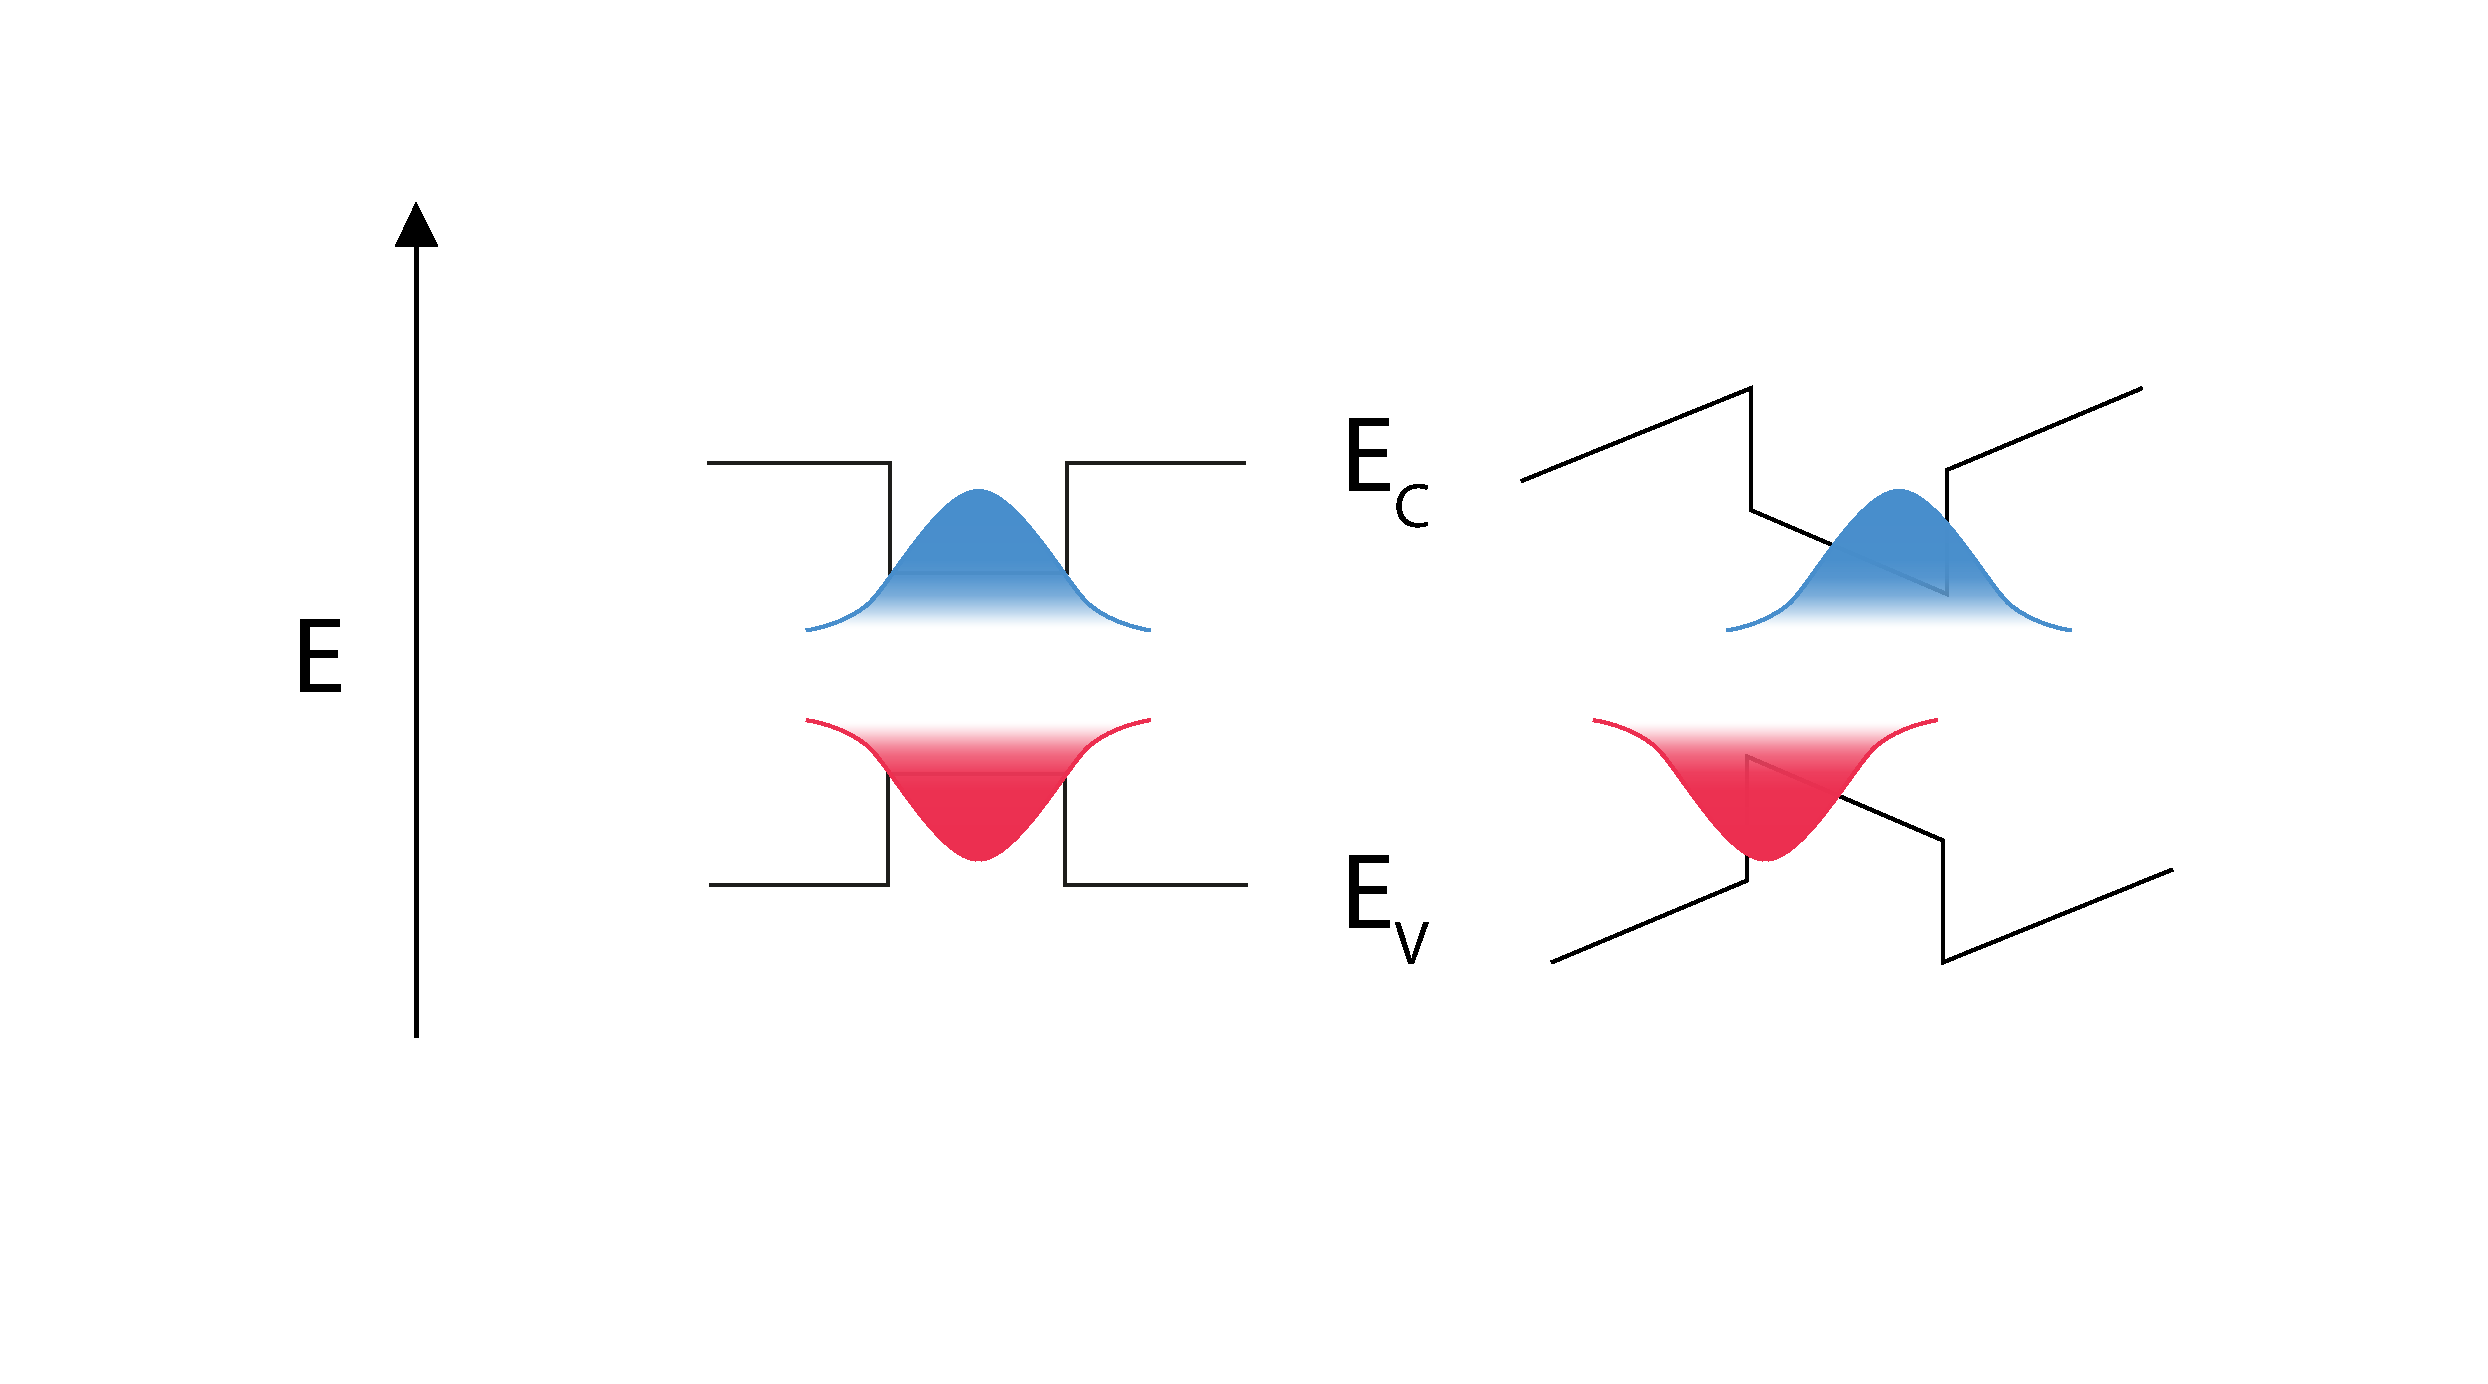
\includegraphics[width=\linewidth]{Bilder/QCSE.pdf}
        \caption{PL-Spektren der Proben ohne Übergitter}
    \end{minipage}% <- sonst wird hier ein Leerzeichen eingefügt
\end{figure}
\vspace{1cm}
\raggedright
\newpage
Die Ursache für die piezoelektrische Polarisation sind die Verspannungen zwischen den in (0001)-Richtung gewachsenen Schichten welche durch die unterschiedlichen thermischen Ausdehnungskoeffizienten und die Gitterfehlanpassung entstehen. Sie wird berechnet nach: 
%
\begin{equation}
    \vec{P}^{pz} = e \cdot \epsilon
\end{equation}
%
	\thispagestyle{fancy}


\section{Metallorganische Gasphasenepitaxie von AlGaN}

Die Metallorganische Gasphasenepitaxie (engl.: matalorganic vapor phase epitaxy, kurz MOVPE) ist die gängigste Methode, um epitaktische Schichten hoher Qualität in ebenfalls hoher Quantität zu wachsen. Es werden gasförmige Ausgangsstoffe in den Reaktor geleitet und dort bei hohen Temperaturen pyrolytisch zerlegt. Ein Teil der auf die Art zerlegten Ausgangsstoffe adsorbiert auf der Oberfläche des verwendeten Substrates und kristallisiert dort schießlich als Epitaxieschicht. 

\section{Substrat}

In der Epitaxie beruhen viele Eigenschaften der aufgewachsenen Schichten auf dem dazu verwendeten Substrat. So sind Gitterfehlanpassung, Defektdichte und die Morphologie wichtige Eigenschaften die durch das Substrat maßgeblich beeinflusst werden. Für AlGaN kann theoretisch auf verschiedene Substrate zurückgegriffen werden und die Vermutung direkt AlGaN basierte Substrate zu verwenden liegt nahe. Dies scheitert allerdings an der besonders hohen Schwierigkeit bei der Herstellung. Daraus resultierend, weisen diese Substrate hohe Defektdichten auf und sind mit sehr hohen Kosten verbunden. Weiterhin ist GaN/Saphir oder GaN als Volumenkristall kommerziell in großen Mengen und hoher Qualität erhältlich, aber aufgrund der Gitterfehlanpassung zwischen zwischen AlN und GaN reißen AlGaN-Schichten mit hohem Aluminiumgehalt auf GaN wegen tensiler Verspannung \cite{problem} . Ein weiterer ungewollter Effekt ist die Absorption von UV-Strahlung ($\lambda \leq 365 \thinspace nm$) im GaN und erlaubt damit keine Verwendung im UV-B und UV-C-Bereich. Daher werden UV-B- und UV-C LEDs und Laserdioden hauptsächlich auf AlN/Saphir oder auf AlN als Volumenkristall gewachsen. Der AlN Volumenkristall weist dabei die kleinste Defektdichte mit $<10^4 \thinspace cm^2$. Jedoch ist die Ausbeute der AlN Substrate zeitaufwendig und teuer. Daher wird für Forschungszwecke auf AlN/Saphir zurückgegriffen und dabei aber eine hohe Defektdichte in kauf genommen. Defekte entstehen dabei im Kristall wegen der hohen Gitterfehlanpassung an der Grenzfläche zwischen AlN und Spahir ~\cite{pohl}. Diese Defekte ziehen sich dabei durch die darauffolgenden aufgewachsenen Schichten. Diese sog. Liniendefekte (engl.: threading dislocation) haben einen wesentlichen Einfluss auf die IQE, wie in Abbildung [\ref{fig:IQEthreadingdisl}] erkennbar. 
%
\begin{figure}[h]
\centering
\begin{minipage}[t]{1\linewidth}
\centering
\includegraphics[width=0.5\linewidth]{Bilder/IQEthreadingdisl.png}
\end{minipage}% <- sonst wird hier ein Leerzeichen eingefügt
\caption{Simulation der IQE einer LED in Abhängigkeit der Versetzungsdichte für einen AlGaN-MQW mit einer Wellenlänge von $280 \thinspace nm$ \cite{0268-1242-26-1-014036}.}
 \label{fig:IQEthreadingdisl}
\end{figure}
\noindent
%
Sie agieren im Kristall als nicht-radiative Rekombinationszentren (engl.: nonradiative recombination center, kurz NRC) und bestimmen somit den Anteil nichtstrahlender Rekombinationsprozesse an der Gesamtheit aller Rekombinationsprozesse. Mit steigender Versetzungsdichte sinkt die IQE des Leuchtdiode und im Bereich zwischen $1\cdot 10^10 \thinspace cm^{-2}$ und $1\cdot 10^8 \thinspace cm^{-2}$ ist eine erhebliche Steigerung zu beobachten. Mittels XRD und TEM wurde gezeigt, dass die Heteroepitaxie von AlN Schichten auf Saphir zu einer Defektdichte von bis zu $2\cdot 10^10 \thinspace cm^{-2}$ führen \cite{zeimeru}.

\section{Defektreduktion durch ELO/AlN-Saphir}

Um die hohe Defektdichte des planaeren AlN/Saphir Substrates zu verringern, ist der übliche Ansatz das sog. epitaktisch laterale Überwachsen (engl.: epitaxial lateral overgrowth) oder kurz ELO. Diese Substrate wurden für alle in dieser Arbeit untersuchten Proben verwendet. 
Als Grundlage für ELO dient ein planares AlN/Saphir Substrat. Dieses wird strukturiert in dem ein Streifenmuster mit einem periodischen Abstand von $3.5 \thinspace \mu m$ reingeätzt wird. Ein weiterer Epitaxie-Schritt mit AlN führt schließlich zum lateralen Überwachsen der Stege an den geätzten Gräben (eng.: voids).
Das Material koalesziert nach einer bestimmten Dicke und bildet schließlich wieder eine bewachsbare Oberfläche. Dabei kommt es zum Auftreten verschiedener Mechanismen wie Verpsannungsabbau und gegenseitig auslöschenden Versetzungen. So ist eine Defektdichte ($\leq 5 \cdot 10^8 \thinspace cm^{-2}$) erreichbar \cite{zeimeru} \cite{MOGILATENKO2014222} \cite{vkueller} \cite{IMURA2007257}. Für eine detaillierte Erklärung sei auf die Doktorarbeit von Viola Küller verwiesen \cite{vkueller}.
	
\thispagestyle{fancy}


\section{Rekombinationsmechanismen}
%
\begin{figure}[h]
\centering
\begin{minipage}[t]{1\linewidth}
\centering
\includegraphics[width=0.8\linewidth]{Bilder/bandrekomb.png}
\end{minipage}% <- sonst wird hier ein Leerzeichen eingefügt
\caption{Durch Einstrahlung eines Photons mit ausreichender Energie können Elektronen vom Valenzband in das Leitungsband angeregt werden. Von dort aus rekombinieren Elektronen und Loch entweder strahlend unter Aussendung eines Photons oder nicht-strahlend.}
 \label{fig:bandrekomb}
\end{figure}
\noindent
In der Photolumineszenzspektroskopie wird Licht als Anregungsquelle von Halbleitermaterialien für die Erzeugung eines Elektron-Loch-Paars benutzt. Dabei wird ein Elektron aus dem Valenzband in das Leitungsband angehoben und wie in Abbildung \ref{fig:bandrekomb} dargestellt ein Loch zurückgelassen. Die Elektronen relaxieren anschließend sehr schnell in das Minimum des Leitungsbandes und analog die Löcher in das Minimum des Valenzbandes. 
\newline
Leitungs- und Valenzband befinden sich im Fall von AlGaN am gleichen $\vec{k}$ -Vektor im reziproken Raum, dem sog. $\Gamma$ -Punkt. Das macht das Materialsystem AlGaN zu einem direkten Halbleiter, was von besonderem Vorteil ist. Denn ein direkter Bandübergang ist die wichtigste Grundlage für eine effiziente halbleiterbasierte Lichtquelle. 
\begin{figure}[htb]
    \centering
    \begin{minipage}[t]{0.49\linewidth}
        \centering
        \includegraphics[width=\linewidth]{Bilder/nonradRekomb.png}
        \caption{Rekombination von Elektron und Loch unter Teilnahme eines Phonons.}
				\label{fig:rekombphoton}
    \end{minipage}% <- sonst wird hier ein Leerzeichen eingefügt
    \hfill
    \begin{minipage}[t]{0.49\linewidth}
        \centering
        \includegraphics[width=\linewidth]{Bilder/radRekomb.png}
        \caption{Strahlende Rekombination von Elektron und Loch und Aussendung eines Photons}
    \end{minipage}
\end{figure}
\noindent
Die Wahrscheinlichkeit einer Anregung und daraufhin folgenden Rekombination unter Aussendung eines Photons ist deutlich höher, da kein Phonon am Prozess beteiligt sein muss (Abb. \ref{fig:rekombphoton}). Die Rekombination kann dennoch auch nicht-strahlend erfolgen, weil epitaktisch gewachsene Halbleitersstrukturen herstellungsbedingt beispielsweise nicht ohne ungewollte Dotierung durch Fremdatome, Versetzungen oder Fehlstellen an Atomgitterplätzen (Vakanzen) gewachsen werden können. Diese fungieren als sogenannte Störstellen und haben diskrete Energieniveaus. 
%
\begin{figure}[h]
    \centering
    \begin{minipage}[t]{0.75\linewidth}
        \centering
        \includegraphics[width=\linewidth]{Bilder/rekbomChannels.png}
        \caption{Übersicht über die beteiligten Rekombinationsprozesse im ABC-Modell, dabei stellt (a) die SRH-Rekombination, (b) die Auger-Rekombination und (c) die strahlende Rekombination dar.}
        \label{fig:rekombChannels}
    \end{minipage}% <- sonst wird hier ein Leerzeichen eingefügt
\end{figure}
\noindent
%
Dazu werden drei Prozesse betrachtet: Zuallererst die nichtstrahlende Rekombination, die durch die Shockley-Read-Hall- (SRH-) Rekombination an Defekten beschrieben und durch den Parameter $A$ berücksichtigt wird ($R_{nonrad} = A \cdot n $). Sie ist linear abhängig von der Ladungsträgerdichte $n$. Sie findet unter der Beteiligung eines Defektniveaus und eines Phonons statt. Der A-Koeffizient ist invers proportional zur SRH-Rekombinations-Lebensdauer. Diese wurde bei defektreichen AlGaN-Schichten im Bereich von einigen $ps$ gemessen. Mit AlGaN-QWs mit Bulk-AlN-Substraten wurden dagegen bereits Lebensdauern im Bereich einiger $ns$ erreicht \cite{1882-0786-4-9-092101} \cite{doi:10.1002/pssc.201100424}.
\newline
Der strahlende Prozess der spontanen Rekombination ist für niedrige Ladungsträgerdichten quadratisch in $n$ und tritt als Zwei-Teilchen Prozess, bei dem Loch und Elektron beteiligt sind ($R_{rad} = B \cdot n^2 $), auf. Dieser wird  mit dem Koeffizienten B beschrieben. Der B-Koeffizient ist stark abhängig vom Design des MQWs wie z.B. der QW-Dicke, QW-Barrieren-Höhe, Verzerrung des AlGaN-QWs und dem Polarisationsfeld im QW \cite{kneissl}. Typische Werte für den B-Koeffizienten liegen in einem Bereich um $2 \cdot 10^{-11} \thinspace cm^3 \thinspace s^{-1}$ \cite{1882-0786-8-2-022104} \cite{1882-0786-4-5-052101}.  
\newline
Der letzte Prozess ist die Auger-Rekombination, die speziell für sehr hohe Anregungsleistungsdichten relevant ist und dann durch die kubische Abhängigkeit stark dominiert ($R_{auger} = C \cdot n^3 $). Dabei gibt ein bereits in das Leitungsband angeregte Elektron seine Energie an ein weiteres Elektron im Leitungsband ab. Dieses relaxiert dann entweder wieder zum Leitungsbandminimum unter Mitwirkung von Phononen oder verlässt bei Oberflächennähe den Kristall. Der letzte Fall bildet die Grundlage für die Auger-Elektronen-Spektroskopie.
Die Größenordnung des C-Koeffizienten für die Gruppe-III-Materialien ist immer noch in Diskussion \cite{8b1c5cf85d5a45e0ae9acca7b03dc349} \cite{doi:10.1063/1.2785135} \cite{doi:10.1002/pssc.200880950} und die Werte für blau-violette LEDs liegen zwischen $1 \cdot 10^{-31}$ und $2 \cdot 10^{-30} \thinspace cm^6 \thinspace s^{-1}$. Die Messmethoden zur Bestimmung des C-Koeffizienten für UV-LEDs sind noch ungenauer \cite{1882-0786-8-2-022104}. Theoretische Modelle sagen aber voraus, dass der C-Koeffizient kleiner werden sollte mit kleiner werdender Wellenlänge \cite{doi:10.1063/1.3570656}.
\newline
Die effektive Rekombination ist somit die Summe aus der strahlenden Rekombination, der nicht-strahlenden Rekombination und der Auger-Rekombination.
\begin{equation}
    R_{eff} = R_{rad} + R_{nonrad} + R_{auger}
    \label{eq:iqe1}
\end{equation}
Der allgemein verwendete Ansatz zur Beschreibung der effektiven Rekombinationsrate $R_{eff}$ (oder auch Generationsrate $G$) wird mit Hilfe der genannten Koeffizienten beschrieben. Er beruht auf der Abhängigkeit der beteiligten Prozesse von der Ladungsträgerdichte $n$ und wird daher auch als ABC-Modell bezeichnet.
\begin{equation}
    R_{eff} (G) = A \cdot n + B \cdot n^2 + C \cdot n^3 
    \label{eq:iqe2}
\end{equation}
Weiter wird angenommen, dass die Anregungsleistungsdichte des Lasers P proportional zu
der Ladungsträger-Generationsrate G ist. Die strahlende Rekombination $R_{rad}$ wird hauptsächlich durch den Überlapp der Wellenfunktionen von Elektronen und Loch im Leitungsband und Valenzband des QW beeinflusst. Dieser wiederum ist stark abhängig vom QCSE (Abb. 
\ref{fig:qcse}) und besonders bedeutend bei heteroepitaktisch gewachsenen Halbleiterstrukturen. 
%

	\newpage
\section{Bestimmung der internen Quanteneffizienz}
\thispagestyle{fancy}
\begin{figure}[h]
    \centering
    \begin{minipage}[t]{0.49\linewidth}
        \centering
        \includegraphics[width=\linewidth]{Bilder/IQEohneDotierungVerschAParams.pdf}
        \caption{Abhängigkeit der internen Quanteneffizienz von der Ladungsträgerdichte für feste Parameter B und C. Der Parameter A wird mit 9 verschiedenen Werten von $0 s^{-1} $ bis $10^9 s^{-1}$ variiert ~\cite{semreich}.}
        \label{fig:abha}
    \end{minipage}
    \hfill
    \begin{minipage}[t]{0.49\linewidth}
        \centering
        \includegraphics[width=\linewidth]{Bilder/BeispielIQEbestimmen.pdf}
        \caption{Photolumineszenzspektrum bei $5K$ und $300K$. Die integrierte Intensität ist die Fläche des jeweiligen Spektrums.}
        \label{fig:beispielint}
    \end{minipage}% <- sonst wird hier ein Leerzeichen eingefügt
\end{figure}
\noindent
Die aktive Region einer idealen LED würde für jedes injizierte Elektron jeweils ein Photon aussenden. 
Das bedeutet, dass die IQE, die nach \cite{schub} wie folgt definiert ist,
\begin{equation}
    IQE = \frac{ \footnotesize \text{Anzahl der Photonen die von der aktiven Zone emittiert werden pro Sekunde}}{ \footnotesize \text{Anzahl der Elektronen die in die LED injiziert werden pro Sekunde}}
\end{equation}
den Wert $1$ annehmen müsste. Die IQE kann somit analog als Verhältnis von strahlender Rekombination und der effektiven Rekombination beschrieben werden. Ausgedrückt durch Ratengleichungen und mit \ref{eq:iqe1} ist die IQE in ihrer einfachsten Form somit
\begin{equation}
    IQE = \frac{B \cdot n^2}{A \cdot n + B \cdot n^2 + C \cdot n^3} = \frac{R_{rad}}{R_{eff}}
\end{equation}
Die IQE kann experimentell mit Hilfe der Photolumineszenzspektroskopie bestimmt werden, indem angenommen wird, dass keine thermisch aktivierten Defekte bei Tieftemperatur vorhanden sind
\begin{equation}
    A \propto e^{\frac{-E_{activation}}{kT}}
\end{equation}
Mit dieser und der Annahme, dass keine Auger Rekombination ($ C \cdot n^3 $) auftritt, ist die IQE bei Tieftemperatur ($ \propto 5K$) gleich 1. Somit kann die IQE als Quotient der integrierten PL Intensität bei Temperatur T und integrierter PL Intensität bei Tieftemperatur ($5K$) beschrieben werden.
\begin{equation}
    IQE(T) = \frac{\text{\textcolor[rgb]{0.65,0.16,0}{Integrierte PL Intensität (T)}}}{ \textcolor[rgb]{0,0,1}{\text{ Integrierte PL Intensität } (T \rightarrow 0 K)} }
    \label{eq:standardiqe}
\end{equation}
Die IQE ist folglich abhängig von der Temperatur, da der Parameter A für die SRH-Rekombination temperaturabhängig ist (Abb. \ref{fig:abha}). 
Um also die IQE bei Raumtemperatur zu bestimmen, wird das Spektrum einer Probe bei 5K und 300K bei ansonsten möglichst gleichen Bedingungen aufgenommen, wie in Abbildung \ref{fig:beispielint} exemplarisch dargestellt ist. Die Intensität in Abhängigkeit der Wellenlänge wird interpoliert, dann integriert und dann das Verhältnis berechnet. 
%
	
\section{Bestimmung der IQE bei Raumtemperatur durch Fitting}

\thispagestyle{fancy}

In diesem Kapitel soll nun eine in \cite{doi:10.1063/1.3100773} und \cite{doi:10.1063/1.4917540} gezeigte Methode zur Bestimmung der IQE durch ein Fitting-Modell für die integrierte Intensität in Abhängigkeit der Ladungsträgerdichte vorgestellt werden. Angefangen mit der Rekombinationasrate, geht das Modell davon aus,
das bei Raumtemperatur Auger-Rekombination nur bei sehr hohen Anregungsleistungsdichten Relevant ist, wegen der kubischen Abhängigkeit der Auger-Rekombination von der Ladungsträgerdichte $n$
\begin{equation}
    G = R_{eff} = A \cdot n + B \cdot n^2
\end{equation}    
G steht hierbei für Generationsrate und beschreibt namentlich die Rate der Ladungsträger die durch Bestrahlung mit dem Laser erzeugt werden und entspricht hierbei der effektiven Rekombinationsrate $R_{eff}$



	\thispagestyle{fancy}

\section{Optische Polarisation und Valenzbandstuktur}
%
\begin{figure}[ht]
    \centering
    \begin{minipage}[t]{0.49\linewidth}
        \centering
        \includegraphics[width=\linewidth]{Bilder/vancebandPlot.png}
        \caption{Die energetische Reihenfolge der Valenzbänder in Abhängigkeit der Kristallfeldaufspaltung. Sichtbar ist der Wechsel der Bandanordnung mit sinkender Kristallfeldaufspaltung und der Effekt des "`anti-crossing"' bei den Bändern gleicher Symmetrie.    }
        \label{fig:auger5k}
    \end{minipage}% <- sonst wird hier ein Leerzeichen eingefügt
    \hfill
    \begin{minipage}[t]{0.49\linewidth}
        \centering
        \includegraphics[width=\linewidth]{Bilder/martinTETM.png}
        \caption{Die Grafik zeigt die sich kontinuierlich ändernde Abstrahlcharakteristik in Abhängigkeit der Polarisation von TE- zu TM~\cite{martingut}.  }
        \label{fig:trueiqe}
    \end{minipage}
\end{figure}
\vspace{0.1cm}
\raggedright
Durch die Prozessierung und die Flip-Chip-Montage kann Licht nur durch die untere, unbewachsene Seite des Saphir-Substrates ausgekoppelt werden. Die Art und Weise der Lichtauskopplung hat einen bedeutenden Einfluss auf die Extraktionseffizienz und damit auf die externe Quantenffizienz(EQE). Durch die Geometrie bestimmt, hängt die Extraktionseffizienz maßgeblich vom Emissionsprofil ab, so dass Licht welches senkrecht zur Quantenfilmebene abgestrahlt wird, die höchste Extraktionseffizienz aufweist. 
Um diese zu optimieren, ist es wichtig die Bandstrukturen zu betrachten.
\newline
Die Valenzbandstrukturen von AlN und GaN unterscheiden sich durch die unterschiedliche anordnung der Bänder. Neben dem Leitungsband gibt es ein durch Spin-Bahn-Wechselwirkung und Kristallfeldenergie dreifach aufgespaltenes Valenzband~\cite{doi:10.1063/1.117689}. Sie werden nach ihrer energetischen Lage als A-,B- und C-Band bezeichnet. In AlN hat das A-Band eine $\Gamma^{L}_{7+}$, das B-Band eine $\Gamma^{L}_{9}$ und das C-Band eine $\Gamma^{L}_{7}$ Symmetrie. Bei GaN hingegen gilt folgende Reihgenfolge:  $\Gamma^{L}_{9}$, $\Gamma^{L}_{7+}$, $\Gamma^{L}_{7}$. Die Ursache für den Symmetriewechsel liegt in der großen negativen Kristallfeldenergie von AlN mit einem Wert von $-221meV$ \cite{PhysRevB.87.235209} im Vergleich zur positiven von GaN mit $12,3meV$ ~\cite{PhysRevB.81.155202}. Bei Raumtemperatur wird, nach der Fermi-Dirac-Verteilung, das oberste Band mit der $\Gamma^{L}_{7+}$-Symmetrie, besetzt und aus Zuständen des $p_z$ bestehend, wird transversal magnetisch (TM) polarisiertes Licht emittiert ist. Die strahlende Rekombination findet demnach überwiegend mit Elektronen und Löchern aus dem A-Band mit $\Gamma^{L}_{7+}$-Symmetrie statt.
In GaN ist das oberste Valenzband am $\gamma$-Punkt mit $\Gamma^{L}_{9}$-Symmetrie . Das elektrische Feld des Lichtes ist senkrecht zur c-Kristallachse und wird durch Übergänge ins A- und B- Band erzeugt~\cite{doi:10.1063/1.3574025}, die aus Zuständen des $p_x$-und $p_y$-Orbitals bestehen. Bei strahlender Rekombination von Elektronen mit den Löchern im A- und B-Band entsteht also überwiegend TE-polarisiertes Licht ~\cite{doi:10.1063/1.3574025} . 
TM polarisiertes Licht kann nicht ausgekoppelt werden, da es nur in der x-y- Ebene (parallel zur Quantenfilmebene) emittiert. Daraus resultierend sinkt die Extraktionseffizienz und damit die EQE. Bei $Al_{x}Ga_{1-x}N$ kommt es mit steigendem Aluminiumgehalt zu einer kontinuierlichen Verschiebung der Valenzbänder und es kommt zum sog. "`anti-crossing"' des $\Gamma^{L}_{7+}$ und $\Gamma^{L}_{7-}$ und resultiert in einer Änderung der Oszillatorstärke und damit der Polarisationseigenschaften ~\cite{doi:10.1063/1.4932651}.  Bedeutet, die Lichtemission ändert sich von hauptsächlich TE-polarisiertem Licht zu TM-polarisiertem Licht. Der genaue Aluminiumgehalt, an dem die Valenzbandkreuzung auftritt, ist noch nicht hinreichend bekannt. Theoretische Betrachtungen sagen für unverzerrtes $Al_{x}Ga_{1-x}N$ einen Kreuzungspunkt bei ca. $7\%$ vorher ~\cite{doi:10.1063/1.3675451}. Durch den starken Einfluss von Verzerrungen auf die Energie der  Valenzbandkante, ist die Polarisation abhängig von der wachsenden biaxialen Verzerrung bei steigendem Aluminiumgehalt. So wurde von Kawanishi et al. experimentell der Wechsel bei einem Aluminiumgehalt von "`75\%"' festgestellt ~\cite{doi:10.1063/1.2410242}. Noch dazu ist ist die Polarisation bei Mehrfachquantenfilmen(engl. multiple quantum wells, kurz MQW) abhängig vom Ladungsträgereinschluss (engl. quantum confinement). Dieser ist hauptsächlich bestimmt durch die Barrierenhöhe und Barrierendicke. Mit kleiner werdender Barrierendicke, steigt der Grad der Polarisation durch den gesteigerten Einfluss des QCSE ~\cite{PhysRevB.84.035305}. 
\newline
\begin{figure}[ht]
    \centering
    \begin{minipage}[t]{0.49\linewidth}
        \centering
        \includegraphics[width=\linewidth]{Bilder/christophPolarisationSimu.png}
        \caption{Simulationsergebnisse des Polarisationsgrades in Abhängigkeit der Aluminiumkonzentration der Barrieren und Quantentöpfe, basierend auf
dem k·p-Modell, für AlGaN-QW mit $1.5nm$-Dicke, die pseudomorph auf ELO-AlN gewachsen wurden. Die gestrichelte Linie zeigt, dass der Wechsel der Polarisation abhängig ist vom Aluminiumanteil in den Barrieren und QWs ~\cite{doi:10.1063/1.4932651} .  }
        \label{fig:simuchr}
    \end{minipage}% <- sonst wird hier ein Leerzeichen eingefügt
    \hfill
    \begin{minipage}[t]{0.49\linewidth}
        \centering
        \includegraphics[width=\linewidth]{Bilder/christophPolarisationSimu1.png}
        \caption{ Ergebnisse der Simulation für die Polarisation in Abhängigkeit von der QW-Dicke(Wellenlänge) und dem Al-Gehalt in den QWs ~\cite{doi:10.1063/1.4932651} .  }
        \label{fig:simu1chr}
    \end{minipage}
\end{figure}
\vspace{0.1cm}
\raggedright
Reich et al. untersuchte unter diesem Zusammenhang die optische Polarisation der Emission von UVC-Leuchtdioden(LEDs) auf Basis von (0001) orientierten $Al_{x}Ga_{1-x}N$-MQWs mit Simulationen und Elektrolumineszenzmessungen ~\cite{doi:10.1063/1.4932651}. Dabei stellte er fest, dass mit zunehmendem Aluminium-Gehalt in den QWs die inplanare-Intensität des TE polarisierten Lichtes gegenüber dem des TM polarisierten Lichts abnimmt, was auf eine Neuordnung der Valenzbänder in $Al_{x}Ga_{1-x}N$ zurückzuführen ist. 
Durch Modellrechnungen, basierend auf dem k·p-Modell, wurde das Design der aktiven Zone von AlGaN MQWs optimiert, wodurch eine erhöhte TE-Polarisation und damit eine höhere Extraktionseffizenz für bottom-emitting LEDs im tiefen UV-Spektralbereich ergibt. Unter der Annahme von schmalen Quantentöpfen, Barrieren mit hohem Aluminium-Gehalt und voll verspanntem Wachstum auf AlGaN-Bulk Substraten wurde bei einer Wellenlänge von nur $239 nm$ eine starke TE-polarisierte Emission beobachtet.
Mit Hilfe der Photolumineszenz lässt sich die Polarisation ebenfalls bestimmen, in dem die Polarisation $\rho$ der Photolumineszenzemission aus der Kante einer Probe mit Hilfe der Gleichung 
\begin{equation}
\rho = \frac{ I_{TE} - I_{TM} }{ I_{TE} - I_{TM} } 
\end{equation}
bestimmt wird. Dabei ist $I_{TE}$ die integrierte Intensität der TE-polarisierten und $T_{TM}$ die Intensität der TM-polarisierten Emission. 
 


	
\chapter{Aufbau}


\thispagestyle{fancy}

\section{Photolumineszenzaufbau}

Für die experimentelle Untersuchung der UV-Photolumineszenz wurde der PL-Aufbau der AG-Kneissl verwendet, den Christoph Reich in der Zeit seiner Masterarbeit aufgebaut und während seiner Promotion erweitert hat~\cite{creich}. 
Als Anregungsquelle für die Photolumineszenz dient ein ArF-Excimerlaser mit einer Wellenlänge von $193 \ nm$ ($6,4 \ eV$). Mit dieser Wellenlänge ist er bestens geeignet für die Überbandanregung von Nitridhalbleitern. 
Des Weiteren bietet der Aufbau die Möglichkeit von temperaturabhängigen Untersuchungen von $5 \ K $ bis $300 K$. Dies ist auch die Grundlage für die Bestimmung der Internen Quanteneffizienz (kurz IQE), die den Großteil der Thematik dieser Arbeit ausmachen wird. 
\newline
Der Laser mit dem Modellnamen  "Xantos" von der Firma Coherent bietet eine maximale Emissionsenergie von $ 5 \ mJ $ und die Frequenz ist bis zu 500 Hz einstellbar bei einer Pulsdauer von $5 \ ns$. 
Durch interne Rückkopplung ist eine Energiestabilisierung möglich, die die Schwankung der Anregungsleistung auf 3 Prozent minimiert. 
\newline
Die Ansteuerung des kompletten Messvorgangs erfolgt durch die Messsoftware von Christoph Reich, entwickelt in der grafischen Programmiersprache "LabView" von Texas Instruments. Mit dieser ist es möglich alle nötigen Einstellungen an Pumpen, Heizern, Laser, Filtern und Spektrometer vorzunehmen, um einen komplett automatisierten Messvorgang zu starten, der nur noch aus Sicherheitsbedingungen überwacht werden muss. Spektren können so mit verschiedenen Parametern wie Position, Anregungsleistungsdichte, Temperatur, Energiebereich und Integrationszeit aufgenommen werden und auch ein Gaswechsel ist möglich.
\newline
Beginnend vom Laser wird im ersten Schritt der Lasterstrahl durch ein Linsensystem bestehend aus einer Zerstreuungs- und Sammellinse aufgeweitet. Dieser Schritt ermöglicht es, die Anregungsleistungsdichte zu verringern, um die am Aufbau beteiligten Gerätschaften nicht mit zu hohen Leistungen zu beschädigen. Damit sind insbesondere die Filterräder gemeint. Mit Hilfe der Filterräder ist es möglich, die Anregungsleistungsdichte 61 stufig zu variieren und somit leistungsdichteabhängige IQE Messungen zu machen. Als nächstes passiert der Strahl ein Linsensystem aus zwei Sammellinsen für eine Strahlverkleinerung. Vor dem Auftreffen des Strahles am Probenhalter im Kryostaten passiert der Strahl noch eine Lochblende. Sie dient der Entfernung achsennaher Strahlen und um bei Bedarf den Strahldruchmesser noch weiter zu verringern. Um den Strahl in Richtung des Probenhalters durch das Fenster im Kryostaten zu lenken, wird ein Spiegel mit einer dielektrischen Beschichtung benutzt. Der Laserstrahl durchdringt die Fenster des Kryostaten, diese sind speziell für eine hohe Transmission in diesem Wellenlängenbereich ausgelegt. Der Kryostat selbst ist horizontal und vertikal verfahrbar um die Messung mehrerer Proben im Probenhalter in einem Vorgang zu ermöglichen. Die Proben werden mit einem Kleber auf dem Probenhalter selbst befestigt, bevor dieser in den Kryostaten geschoben wird. 
Die Anregung der Proben mit dem Laserstrahl führt zur Proben spezifischen Emission von Licht. Diese wird von einer Linse im Strahlengang vor dem Detektor eingefangen und von einer zweiten Linse eingefangen die auf den Monochromatorspalt fokussiert ist.


	
\thispagestyle{fancy}

\section{Bestimmung der Degradation des UV Quarzglases}
%
\begin{figure}[htb]
  \centering
  \begin{minipage}[t]{0.49\linewidth}
      \centering
      \includegraphics[width=\linewidth]{Bilder/uvsilicaDegradation.png}
      \caption{Vom Hersteller angegebene wellenlängenabhängige Transmission vor und nach Degradation durch Bestrahlung.}
      \label{fig:degra}
  \end{minipage}
\end{figure}
\noindent
Da die Messung der Anregungsleistungdichte erfolgt, bevor das Laserlicht die Probe durch das UV-Quarzglas im Kryostaten trifft, ist es wichtig den Transmissionsverlust zu bestimmen, um die realen Werte für die Anregungsleistungsdichte zu kennen (Die Anregungsleistungsdichte, die bei der Probe ankommt). Der Kryostat besitzt vier Fenster, bestehend aus UV-Quarzglas, das besonders transparent im UV-Wellenlängenbereich ist. Durch diese Fenster dringt das Laserlicht in den Probenhalter ein. Von diesen Fenstern war und ist eines in dauerhaftem Gebrauch. Wie in Abbildung \ref{fig:degra} zu sehen ist, weisen die Fenster aber mit der fortlaufender Bestrahlung Degradation auf. So nimmt laut Hersteller durch Degradation die Transmission von 90 Prozent bis auf ca. 75 Prozent für eine Wellenlänge von 193 nm ab.
\newline
Um nun den Transmissongrad zu bestimmen, wurde der Probenhalter aus dem Kryostat entfernt, damit das Laserlicht ungehindert durch zwei parallel liegende Fenster durchdringen kann, um so auch die Anregungsleistungsdichte des Laserlichtes nach durchdringen des letzten Fenster messen zu können. So konnte die Anregungsleistungsdichte vor dem Eintreten und nach dem Austreten in den Kryostaten bestimmt werden. 
\newline
Dies wurde einmal bei den parallel liegenden unbenutzten Fenstern durchgeführt. Davon ausgehend, dass beide Fenster, da unbenutzt, den gleichen Transmissionsgrad haben, kann darauf zurückgeschlossen werden, dass ein unbenutztes Fenster einen Transmissionsgrad von 59 Prozent aufweist. Dies weicht um ca. 10 Prozent von der Herstellerangabe ab, die aber nicht die Reflektion im Kryostaten miteinbezieht. 
%
\begin{figure}[htb]
  \centering
  \begin{subfigure}{0.40\textwidth}
    \centering
    \includegraphics[width=0.9\linewidth]{Bilder/uvsilicavergleich.pdf}
    \caption{PL Intensität in Abhängigkeit der Anregungsleistungsdichte mit den benutzten und unbenutzten Fenstern}
    \label{fig:sub1}
  \end{subfigure}%
  {\LARGE$\xrightarrow{\cdot 0,44}$}
  \begin{subfigure}{0.40\textwidth}
    \centering
    \includegraphics[width=0.9\linewidth]{Bilder/uvsilicaVergleichSkaliert.pdf}
    \caption{Die Anregungsleistungsdichte des unbenutzten Fensters mit den rechnerisch bestimmten 0,44 skaliert}
    \label{fig:sub2}
  \end{subfigure}
  \caption{}
  \label{fig:vergleichSkaliert}
\end{figure}
\newline
Um den Transmissionsgrad des benutzten Fensters zu bestimmen, wurde die Transmission durch das benutzte und dem parallel liegende unbenutzte Fenster gemessen. Mit dem Wissen, dass der Transmissionsgrad durch das unbenutzte Fenster bei 59 Prozent ($T_{unb} = 0,59$) liegt, kann die Transmission durch das benutzte Fenster auf 26 Prozent ($T_{ben} = 0,26$) berechnet werden. 
Davon ausgehend, dass die Transmission bei höheren Wellenlängen (Emission) gleich und bei beiden Fenstern ähnlich ist,
%
\begin{equation}
  F_{skal} = \frac{ T_{ben} }{ T_{unb} } = 0,44\label{eq11}
\end{equation}
%
kann der Skalierungsfaktor mit für die Anregungsleistungsdichte auf 0.44 bestimmt werden. Dies bedeutet, dass durch Degradation die Transmission auf 44 Prozent der ursprünglichen Transmission gesunken ist.
\newline
Dies bestätigt sich auch durch die Gegenüberstellung in  Abbildung \ref{fig:vergleichSkaliert}. Somit ist durch die zeitliche Degradation die Transmission auf 44 Prozent der ursprünglichen gesunken. Dies bestätigt im Umkehrschluss, dass von der ausgehenden Anregungsleistungsdichte, die vor dem Kryostaten gemessen wird, durch die geringe Transmission der Fenster und Reflektion im und außerhalb des Kryostaten nur ca. 26 Prozent des vom Laser emittierten Lichtes bei der Probe ankommen. 
	\section{Aufbau: Erweiterung der Filterkombinationen}
\thispagestyle{fancy}

Im Zuge dieser Arbeit wurden für eine Erhöhung der Messpunkte und Verringerung von Rauschen bei der leistungsdichteabhängigen Messung der IQE die Anzahl der Filterkombination erhöht. Dafür wurden die alten zwei Filterräder durch drei neue ersetzt. 
%
\begin{figure}[ht!]
    \centering
    \begin{minipage}[t]{1\linewidth}
        \centering
        \includegraphics[width = 0.49\linewidth]{Bilder/AuswertungNovemeberKorr1VergleichFilter.pdf}
        \caption{Vergleich der Messung von insgesamt 5 ähnlichen Proben. 3 Proben (blau) wurden mit dem alten Setup gemessen. 2 Proben (grün, durchgezogene Linie) wurden mit dem neuen Setup gemessen. Die Präzision in tieferen Anregungsleistungsdichtenbereichen ist für das neue Setup deutlich erhöht. Das Rauschen fällt ebenfalls deutlich geringer aus. }
        \label{fig:vergleichFilter}
    \end{minipage}
\end{figure}
%
\newpage
Durch die erhöhte Anzahl möglicher Filterkombinationen ist es möglich, statt nur 27 verschiedene Messpunkte 61 zu nehmen. Speziell der Bereich der geringen Anregungsleistungsdichten kann so besser aufgelöst werden und das Rauschen wurde im Allgemeinen stark verringert \ref{fig:vergleichFilter}. 
%

	\newpage

\section{Einfluss der Auger-Rekombination auf die IQE}
%
\begin{figure}[h]
    \centering
    \begin{minipage}[t]{0.49\linewidth}
        \centering
        \includegraphics[width=\linewidth]{Bilder/AugerBei5K.pdf}
        \caption{Die Grafik zeigt die Abhängigkeit der internen Quanteneffizienz von der Ladungsträgerdichte für feste Paramater B und C unter Variation des A Parameters und Beachtung des Einflusses einer Silizium-Dotierung.}
        \label{fig:auger5k}
    \end{minipage}% <- sonst wird hier ein Leerzeichen eingefügt
    \hfill
    \begin{minipage}[t]{0.49\linewidth}
        \centering
        \includegraphics[width=\linewidth]{Bilder/NormierteKorrgierteIQE5K.pdf}
        \caption{Die Grafik zeigt die normierte korrigierte IQE bei 5K nach Gleichung [\ref{eq:iqetrue5k}] }
        \label{fig:trueiqe}
    \end{minipage}
\end{figure}
\vspace{1cm}
\raggedright
Das bisher benutzte Modell zur Bestimmung der PL-IQE ging davon aus, dass bei Tieftemperatur keine Auger-Rekombination (Gleichung) vorkommt, aber wie in Abb. [\ref{fig:auger5k}] deutlich zu erkennen, nimmt der Verlauf der PL-Intensität in doppeltlogarithmischer Darstellung gegenüber der Anregungsleistungsdichte (die direkt proportional zur Ladungsträgerdichte ist), im Bereich höherer Anregungsleistungen (entsprechend höheren Ladungsträgerdichten) deutlich ab und weist keinen linearen Verlauf mehr auf, den er aber durch eine allein quadratische Abhängigkeit (in doppeltlogarithmischer Darstellung linear) haben sollte. Dies zeigt, dass die IQE nicht, wie bisher angenommen, immer bei 100 Prozent liegt, sondern auch bei Tieftemperatur Anregungsleistungsdichte abhängig ist. Um dies zu berücksichtigen, wird nun die IQE bei 5K definiert als:
%
\begin{equation}
    IQE_{true}(T = 5K, A_{exc}) = \frac{ \frac{I_{pl}(T,A_{exc}) }{A_{exc} } } { \lvert \lvert \frac{I_{pl}(T,A_{exc})}{A_{exc}} \lvert \lvert_{max} }
    \label{eq:iqetrue5k}
\end{equation}
%
Wobei $I_{pl}(A_{exc})$ die von der Anrengungsleistungsdichte $A_{exc}$ und Temperatur $T = 5K$ abhängige integrierte PL-Intensität ist. Die integrierte PL-Intensität wird durch die Anregungsleistungsdichte dividiert und auf das Maxmimum normiert, so dass das Maximum der IQE bei $5K$ bei der geringsten Anregungsleistungdichte mit der geringsten Auger-Rekombination liegen sollte. Um nun die IQE bei Raumtemperatur zu bestimmen, wird die nach dem alten Verfahren ermittelte IQE multipliziert mit den neu ermittelten Werten passend zur Anregungsleistungsdichte. 
%
\begin{equation}
    IQE(T, A_{exc}) = \frac{IQE(T,A_{exc})}{IQE(5K,A_{exc})} \cdot IQE_{true}(5K,A_{exc})
\end{equation}
%
Die IQE bei $5K$ dient hierbei also als Skalierungsfaktor, der den Einfluss der Auger-Rekombination bei Raumtemperatur korrigiert. Somit fällt im Vergleich insbesondere auf, dass die Skalierung bei den kleinsten Anregungsleistungsdichten am geringsten Einfluss hat und mit steigender Anregungsleistungsdichte kubisch steigt, so dass die nach dem alten Verfahren ermittelten IQE-Werte bei höheren Anregungsleistungsdichten deutlich nach unten korrigiert werden müssen. 
%
\begin{figure}[h]
    \centering
    \begin{minipage}[t]{0.49\linewidth}
        \centering
        \includegraphics[width=\linewidth]{Bilder/StandardIQE300K.pdf}
        \caption{Die Grafik zeigt die Abhängigkeit der internen Quanteneffizienz von der Ladungsträgerdichte für feste Paramater B und C unter Variation des A Parameters und Beachtung des Einflusses einer Silizium-Dotierung.}
        \label{fig:standiqe300k}
    \end{minipage}% <- sonst wird hier ein Leerzeichen eingefügt
    \hfill
    \begin{minipage}[t]{0.49\linewidth}
        \centering
        \includegraphics[width=\linewidth]{Bilder/KorrigierteIQE300K.pdf}
        \caption{Die Grafik zeigt die normierte korrigierte IQE bei 5K nach Gleichung [\ref{eq:iqetrue5k}] }
        \label{fig:trueiqe300k}
    \end{minipage}
\end{figure}
\vspace{1cm}
\raggedright
%
fssfsdf

	\thispagestyle{fancy}
\justifying
\chapter{Untersuchung des MQW-Designs von AlGaN-UVC-Heterostrukturen}
\label{chap:mqw}
\section{Einleitung}
Dieses Kapitel widmet sich der Untersuchung von AlGaN-MQWs in UVC-LED-Heterostrukturen verschiedener Dicken mit dotierten und undotierten Barrieren. Mit Hilfe der UV-Photolumineszenz sollen der Einfluss der variierenden QW-Dicke und Dotierung auf die interne Quanteneffizienz und die Emissionsenergien untersucht werden um das MQW-Design zu optimieren.
\begin{figure}[H]
  \centering
  \begin{minipage}[t]{0.49\textwidth}
    \centering
    \includegraphics[width=\textwidth]{Bilder/MQWdickenSerie/undotiert}
		\caption{Aufbau der untersuchten MQW-Proben ohne dotierte Barrieren.}
    \label{fig:undotiert}
  \end{minipage}
	\hfill
  \begin{minipage}[t]{0.49\textwidth}
    \centering
    \includegraphics[width=\linewidth]{Bilder/MQWdickenSerie/dotiert}
		\caption{Aufbau der untersuchten MQW-Proben mit dotierten Barrieren.}
    \label{fig:dotiert}
  \end{minipage}
\end{figure}
\noindent 
Der Aufbau der Proben ohne dotierte Barrieren ist in Abbildung \ref{fig:undotiert} zu sehen.
Die aktive Zone setzt sich aus zwei $5 \thinspace nm$ dicken $ Al_{0.81}Ga_{0.19}N$-Barrieren zwischen den drei $ Al_{0.60}Ga_{0.40}N$ QWs mit variierender Dicke $d$ mit $d=1,2,3,4 \thinspace nm$. Sie befindet sich zwischen zwei $40 \thinspace nm$ dicken $ Al_{0.81}Ga_{0.19}N$-Barrieren von der eine die oberste Schicht darstellt. Darunter folgt eine AlN ($100\%$)-Bufferschicht die auf einem ELO-AlN/Saphir Substrat aufgewachsen wurde. 
\newline
Abbildung \ref{fig:dotiert} zeigt den Aufbau der Proben mit dotierten Barrieren. Die aktive Zone setzt sich aus zwei $5$nm dicken und Si-dotierten $ Al_{0.83}Ga_{0.17}N:Si$-Barrieren zwischen den drei $ Al_{0.72}Ga_{0.36}N$ QWs mit variierender Dicke $d$ mit $d=0.5,1.0,2.2,4 \thinspace nm$. Diese befindet sich zwischen zwei $40 \thinspace nm$ dicken und Si-dotierten $ Al_{0.81}Ga_{0.19}N:Si$-Barrieren von der eine die oberste Schicht darstellt. Darunter folgt eine AlN ($100\%$)-Bufferschicht die auf einem ELO-AlN/Saphir Substrat aufgewachsen wurde. 
\section{Ergebnisse}
Für die experimentelle Untersuchung wurden Photolumineszenzmessungen bei Tieftemperatur gemacht und die Spektren aufgenommen.
Die Abbildungen \ref{fig:undotiertSpektrumn} und \ref{fig:dotiertSpektrumn} zeigen die aufgenommenen Spektren.
Es ist deutlich zu erkennen, dass mit sinkender QW-Dicke $d$ die Emissionsenergie steigt.
\begin{figure}[H]
  \centering
  \begin{minipage}[t]{0.45\textwidth}
    \centering
    \includegraphics[width=\textwidth]{Bilder/MQWdickenSerie/spektrumUndotiert}
		\caption{PL-Spektren der untersuchten MQW-Proben ohne dotierte Barrieren.}
    \label{fig:undotiertSpektrumn}
  \end{minipage}
	\hfill
  \begin{minipage}[t]{0.45\textwidth}
    \centering
    \includegraphics[width=\linewidth]{Bilder/MQWdickenSerie/spektrumDotiert}
		\caption{PL-Spektren der untersuchten MQW-Proben mit dotierten Barrieren.}
    \label{fig:dotiertSpektrumn}
  \end{minipage}
\end{figure}
\noindent 
Die Gründe hierfür sind die Übergangsenergien die mit steigender QW-Dicke \cite{doi:10.1063/1.371241} sinken. 
Die Emissionsenergien fallen im Vergleich beider Serien deutlich unterschiedlich aus, da die aktiven Zonen unterschiedliche Zusammensetzungen in den Barrieren und QWs (siehe Abb. \ref{fig:undotiert} und \ref{fig:dotiert}) haben. 
\newline
In den Abbildungen \ref{fig:undotiertint} und \ref{fig:dotiertint} ist die integrierte Intensität in Abhängigkeit der Anregungsleistungsdichte bei Tieftemperatur für die Proben mit undotierter und dotierter Barriere in doppeltlogarithmischer Darstellung dargestellt.
\begin{figure}[H]
  \centering
  \begin{minipage}[t]{0.49\textwidth}
    \centering
    \includegraphics[width=\textwidth]{Bilder/MQWdickenSerie/intTTundotiert.png}
		\caption{Integrierte Intensität in doppeltlogarithmischer Darstellung in Abhängigkeit der Anregungsleistungsdichte bei Tieftemperatur für die Proben mit undotierter Barriere.}
    \label{fig:undotiertint}
  \end{minipage}
	\hfill
  \begin{minipage}[t]{0.49\textwidth}
    \centering
    \includegraphics[width=\linewidth]{Bilder/MQWdickenSerie/intTTdotierte.png}
		\caption{Integrierte Intensität in doppeltlogarithmischer Darstellung in Abhängigkeit der Anregungsleistungsdichte bei Tieftemperatur für die Proben mit dotierter Barriere.}
    \label{fig:dotiertint}
  \end{minipage}
\end{figure}
\noindent 
Im Bereich geringer Anregungsleistungsdichten zeigt sich für beide Serien eine lineare Steigung (gestrichelte Linie) die mit zunehmender Anregungsleistungsdichte ein nichtlinearen Verlauf annimmt der auf die Auger-Rekombination zurückzuführen ist (siehe Kapitel \ref{chap:auger}).
Die integrierten Intensitäten befinden sich für die Proben mit undotierter Barriere bei Tieftemperatur für alle QW-Dicken auf dem selben Niveau.
\newline
Die Proben mit einer QW-Dicke von $3,0 \thinspace nm$ und $4,0 \thinspace nm$ leuchten am hellsten und darauf folgen die Proben mit $2.0 \thinspace nm$ und $1.0 \thinspace nm$  QW-Dicke. Die Unterschiede sind aber marginal und im Rahmen der Streuung, die durch die unterschiedlichen Fokussierungen und Positionen im PL-Aufbau zu erwarten sind. Gleiches gilt für die Proben mit dotierter Barriere. Dort fallen die Proben mit QW-Dicken von $2.2 \thinspace nm$ und $4.4 \thinspace nm$ deutlicher ab, jedoch in einem unbedenklichen Maß.   
\begin{figure}[H]
  \centering
  \begin{minipage}[t]{0.49\textwidth}
    \centering
    \includegraphics[width=\textwidth]{Bilder/MQWdickenSerie/PeakEnergieUndotiert.png}
		\caption{Peak-Emissionsenergie in Abhängigkeit der Anregungsleistungsdichte bei Tieftemperatur der untersuchten MQW-Proben ohne dotierte Barrieren.}
    \label{fig:undotiertpeak}
  \end{minipage}
	\hfill
  \begin{minipage}[t]{0.49\textwidth}
    \centering
    \includegraphics[width=\linewidth]{Bilder/MQWdickenSerie/PeakEnergieDotiert.png}
		\caption{Peak-Emissionsenergie in Abhängigkeit der Anregungsleistungsdichte bei Tieftemperatur der untersuchten MQW-Proben mit dotierten Barrieren.}
    \label{fig:dotiertpeak}
  \end{minipage}
\end{figure}
\noindent 
Für die Proben mit undotierten Barrieren ist in Abbildung \ref{fig:undotiertpeak} zu erkennen, dass mit steigender Anregungsleistungsdichte die Peak-Emissionsenergie steigt. Der Grund hierfür ist das Screening des QCSE \cite{doi:10.1063/1.1763211}. Dieser Effekt wird größer mit kleiner werdender QW-Dicke, weil mit kleinerer QW-Dicke die Auswirkung des QCSE geringer ausfällt. Dies bedeutet, dass eine geringere Ladungsträgerdichte im QW notwendig, um die Bandverbiegung und damit die Separation der Elektron- und Lochwellenfunktion aufzuheben. 
\newline
Damit einhergehend ist die Verschiebung der Peak-Emissionsenergien bei der Probe mit einer QW-Dicke von $5 \thinspace nm$ von $4,65 \thinspace eV$bei der geringsten Anregungsleistungsdichte zu $4,77 \thinspace eV$ bei der höchsten Anregungsleistungsdichte am stärksten. 
\newline 
Die Probe mit einer QW-Dicke von $1 \thinspace nm$ zeigt dagegen keine Verschiebung der Peak-Emissionsenergien. Dies bestätigt, dass für kleine Dicken $d$, eine geringere Ladungsträgerdichte für das Screening des QCSE notwendig werden.
\newline
Die Proben mit dotierten Barrieren zeigen ein ähnliches Verhalten, so sind die Peak-Emissionsenergien für die Proben mit einer QW-Dicke von 
$1,0 \thinspace nm$, $2,2 \thinspace nm$ und $4,4 \thinspace nm$ nahezu konstant über den ganzen Bereich der Anregungsleistungsdichte.
Der Grund hierfür könnte sein, dass bereits eine höhere Anzahl an Ladungsträgern durch die Dotierung zur Verfügung stehen, die zusätzlich zur  externen Anregung dazu beitragen den Effekt des QCSE zu reduzieren.
\newline
Auffällig ist, dass die Emissionsenergie der Probe mit der geringsten QW-Dicke von $0,5 \thinspace nm$ sich mit steigender Anregungsleistungsdichte hin zu kleineren Energie verschiebt. Die Gründe für dieses Verhalten sind bisher unklar.
\begin{figure}[H]
  \centering
  \begin{minipage}[t]{0.49\textwidth}
    \centering
    \includegraphics[width=\textwidth]{Bilder/MQWdickenSerie/IQEundotiert.png}
		\caption{IQE in Abhängigkeit der Anregungsleistungsdichte bei Raumtemperatur der untersuchten MQW-Proben ohne dotierte Barrieren.}
    \label{fig:undotiertIQE}
  \end{minipage}
	\hfill
  \begin{minipage}[t]{0.49\textwidth}
    \centering
    \includegraphics[width=\linewidth]{Bilder/MQWdickenSerie/IQEdotiert.png}
		\caption{IQE in Abhängigkeit der Anregungsleistungsdichte bei Raumtemperatur der untersuchten MQW-Proben.}
    \label{fig:dotiertIQE}
  \end{minipage}
\end{figure}
\noindent 
Die Ergebnisse der IQE bei Raumtemperatur für die Proben ohne und mit dotierten Barrieren sind in den Abbildungen 
\ref{fig:undotiertIQE} und \ref{fig:dotiertIQE} zu sehen. Für beide Probenserien zeigt sich, dass aufgrund des QCSE die IQE für weite QWs 
($3.0 -4.0  nm$) geringer ausfällt. Ebenso für besonders geringe Dicken ($0.5\thinspace nm$), bedingt durch den schlechteren Ladungsträgereinschluss. Die höchste IQE wird für QW-Dicken von $1.0 \thinspace nm- 2.2 \thinspace nm$ gemessen. Die Proben ohne dotierte mit QW-Dicken von $1.0 \thinspace nm$ und $2.0\thinspace nm$ haben beide eine IQE von ca. $0,145$ bei höchster Anregungsleistungsdichte.
\newline
Die Proben mit dotierten Barrieren und QW-Dicken von $1.0 \thinspace nm$ und $2.2\thinspace nm$ haben beide eine IQE von ca. $0,121$ bei höchster Anregungsleistungsdichte. 
\newline
Anhand der Ergebnisse für die Proben mit dotierten Barrieren ist zu erkennen, dass die Si-dotierung einen deutlichen Einfluss auf den Verlauf der IQE hat. So ist die Ordinate der IQEs für diese Proben deutlich höher, wie Abbildung \ref{fig:dotiertIQE} zeigt. Die Dotierung führt sichtbar zu höheren IQEs bei geringen Anregungsleistungsdichten. Die Steigung mit anwachsender Anregungsleistungsdichte ist aber im Vergleich geringer, sodass die IQEs für beide Serien ungefähr den selben Wert im Bereich der hohen Anregungsleistungsdichten einnehmen. 
\newline
Der Grund für dieses unterschiedliche Verhalten ist durch den Effekt der Dotierung auf den QCSE zu erklären. Durch die Si-Dotierung werden Ladungsträger in die Struktur gebracht, die neben der durch Anregung extern zugeführten Ladungsträgerdichte, zu einer zusätzlichen Abschirmung der Polarisationsfelder führen. Dieser Effekt ist am deutlichsten bei geringen Anregungsleistungsdichten zu sehen und hebt sich im Bereich großer Anregungsleistungsdichten auf, da die durch Anregung generierte Ladungsträgerdichte den Effekt des Screenings deutlich dominiert.

\iffalse
\section{Einfluss der Siliziumdotierung auf die IQE}

Um die Unterschiede in der IQE für dotierte- und undotierte Barrieren zu klären, soll nun das ABC-Modell erweitert werden, um den Effekt der Dotierung mit einzubeziehen. 
Das ABC-Modell stellt nur eine Vereinfachung dar und berücksichtigt nicht alle vorkommenden Effekte wie beispielsweise Lokalisierung, Screening durch Ladungsträger und Dotierung. 
Der Effekt der Dotierung spielt dabei eine besonders wichtige Rolle, da eine Si-Dotierung für das erreichen einer hohen Leitfähigkeit üblich in UV-LEDs ist \cite{doi:10.1063/1.1492316}.
Nach \cite{schub} soll mit Hilfe der Ratengleichungen gezeigt werden, dass sich mit der Annahme einer Dotierung,
der Anteil der strahlenden Rekombination ändert.
\newline
\begin{figure}[H]
    \centering
    \begin{minipage}[t]{0.49\linewidth}
        \centering
        \includegraphics[width=\linewidth]{Bilder/IQEohneDotierungVerschAParams.pdf}
        \caption{Die Grafik zeigt}
        \label{fig:iqenorm}
    \end{minipage}% <- sonst wird hier ein Leerzeichen eingefügt
    \hfill
    \begin{minipage}[t]{0.49\linewidth}
        \centering
        \includegraphics[width=\linewidth]{Bilder/IQEmitDotierungVerschAParams.pdf}
        \caption{Die Grafik zeigt  }
        \label{fig:iqedot}
    \end{minipage}
\end{figure}
\vspace{0.1cm}
\noindent
Jeder dotierte oder undotierte Halbleiter hat zwei Arten von Ladungsträgern, Elektronen und Löcher.
Im Gleichgewicht, bedeutet ohne externe Anregung durch Absorption von Licht oder Injektion von Elektronen, ist das Produkt von Elektronen- und Lochkonzentration eine konstante Größe.
\begin{equation}
    n_0 \cdot p_0 = n_i^2
    \label{eq:constant}
\end{equation}
Hierbei sind $n_0$ und $p_0$ die Elektron- und Lochkonzentration unter Gleichgewichtsbedingung und $n_{i}$ damit die intrinsische Ladungsträgerkonzentration.
Werden zusätzlich die durch Anregung erzeugten Ladungsträger betrachtet, so ist die Gesamtladungsträgerkonzentration gegeben als Summe der Anregungs- und Gleichgewichtsladungsträger. 
\begin{equation}
    n_{ges} = n_0 + n \medspace \text{und} \medspace  p_{ges} = p_0 +  n 
\end{equation}
Hierbei sind $ n$ und $p$ die Anregungsladungsträger. 
Die Anzahl der stattfindenden Rekombination zwischen Elektronen und Löchern sind direkt proportional zur Elektronen-und Ladungsträgerkonzentration, so gilt, $R \propto n \cdot p $. Mit einer Proportionalitätskonstante, wird die Rekombinationsrate pro Zeit und Volumen definiert als
\begin{equation}
    R = - \frac{dn_{ges}}{dt} = - \frac{dp_{ges}}{dt} = B \cdot n_{ges} \cdot p_{ges}
\end{equation}
Weil Elektronen und Löcher bei Anregung paarweise erzeugt werden und verschwinden (durch Rekombination), gilt
\begin{equation}
    \label{eq:gleich}
    n(t) =  p(t)
\end{equation}
Die radiative Rekombinationsrate wird dann mit $p_{0} = 0$ und Gleichung \ref{eq:gleich} zu
\begin{align}
\begin{split}
    R_{rad} &= B \cdot (n_0 + n)  \cdot (p_0 + p) ,
    \\
    R_{rad} &= B \cdot (n_0 + n) \cdot (n) ,
    \\
    R_{rad} &= B \cdot n^2 + B \cdot n \cdot n_0
\end{split}
\end{align}
Dabei beschreibt $n_{0}$ die Ladungsträgerkonzentration durch die Silizumdotierung. 
Somit wird die IQE zu:
\begin{equation}
    IQE = \frac{B \cdot n^2 + B \cdot n \cdot n_{0}}{A \cdot n + B \cdot n^2  + B \cdot n \cdot n_{0}+ C \cdot n^3} 
    \label{eq:dopediqe}
\end{equation}
Und hat einen enormen Einfluss auf die Ordinate, wie in Abb. \ref{fig:iqedot} zu sehen ist und zeigen damit im Vergleich mit der experimentell ermittelten IQE in Abbildung \ref{fig:dotiertIQE} für die Serie mit dotierten Barriere einen ähnlich Verlauf.

\fi

\section{Ergebnisse der Simulationen}
\begin{figure}[H]
  \centering
  \begin{minipage}[t]{0.49\textwidth}
    \centering
    \includegraphics[width=\textwidth]{Bilder/MQWdickenSerie/Simu1.png}
		\caption{Simulation der Elektron- und Lochwellenfunktion im Bändermodell mit QW in einem Bereich von $-4$ bis $4 \thinspace nm$ für verschiedene Dicken. Simulation von Christoph Reich.}
    \label{fig:simu1}
  \end{minipage}
	\hfill
  \begin{minipage}[t]{0.49\textwidth}
    \centering
    \includegraphics[width=\linewidth]{Bilder/MQWdickenSerie/Simu2.png}
		\caption{Wellenfunktion Überlappintegral in Abhängigkeit der QW-Dicke. Simulation von Christoph Reich.}
    \label{fig:simu2}
  \end{minipage}
\end{figure}
\noindent 
Abbildung \ref{fig:simu1} und \ref{fig:simu2} und zeigen Modellberechnungen von Christoph Reich basierend auf der \textbf{k$\cdot$p}-Theorie für variierende QW-Dicken. In Abbildung \ref{fig:simu1} sind die Elektron und Lochwellenfunktion im Bändermodell für die vier verschiedenen Dicken von 
$d=0.5,1.0,2.2,4 \thinspace nm$ dargestellt. 
\newline
Dazu passend zeigt Abbildung \ref{fig:simu2} die zugehörigen Überlappintegrale der Wellenfunktionen.
Das Überlappintegral ist ein Maß für die strahlende Rekombination. Daraus folgt, dass je höher der Wert des Überlappintegrals ist, umso größer ist der Anteil der strahlenden Rekombination. 
Somit ist für QW-Dicken von $1.0 \thinspace nm- 2.0 \thinspace nm$ der höchste B-Paramater für die strahlende Rekombination zu erwarten und
bei Annahme dass Auger-Rekombination und nicht-strahlende Rekombination gleich bleiben auch die höchsten IQEs und bestätigt damit die experimentellen Ergebnisse.
\newline
Des Weiteren bestätigt die Simulation, dass für eine QW-Dicke von $0,5 \thinspace nm$ die IQE im Vergleich geringer ausfällt, da das Überlappintegral durch den geringeren Ladungsträgereinschluss am kleinsten ausfällt. 

\section{Zusammenfassung}

Die Ergebnisse dieses Kapitels zeigen, dass die QW-Dicke einen eindeutigen Einfluss auf die Rekombination und damit auf die IQE hat. Es wurde experimentell gezeigt und durch \textbf{k$\cdot$p}-Simulationen bestätigt, dass QW-Dicken von $1.0 \thinspace nm- 2.2 \thinspace nm$ die höchsten IQEs und somit das beste Verhältnis zwischen Ladungsträgereinschluss und Screening liefern. 
\newline
Die gemessenen IQEs für die Proben mit dotierten und undotierten Barrieren liegen zwischen $0,121$ und $0,145$ und sind damit auf einem ähnlichen Niveau. Es zeigte sich, dass eine Dotierung in den Barrieren im Bereich geringer Anregungsleistungsdichten zu höheren IQEs führt, diese jedoch im Vergleich weniger stark ansteigen in Abhängigkeit der Anregungsleistungsdichte.
\newline
Weiter wurde gezeigt, dass die Emissionsenergien der undotierten Proben durch das Screening des QCSE mit zunehmender Ladungsträgerdichte steigen und für die Serie mit dotierten Barrieren konstant bleiben, aufgrund der größeren Anzahl an Ladungsträgern die den QCSE reduzieren.

	
\thispagestyle{fancy}
\justifying
\chapter{Untersuchung optisch gepumpter Laserstrukturen auf unterschiedlichen Templates}
\label{chap:offcut}

\section{Einleitung}
Dieses Kapitel widmet sich der Untersuchung zweier Probenreihen von optisch gepumpten Laserstrukturen, die aus Rezepten aus zwei unterschiedlichen Serien stammen. Die beiden Serien unterscheiden sich im wesentlichen dadurch, dass sie mit(Serie 2) und ohne Übergitter(Serie 1) gewachsen wurden. Sie haben alle eine aktive Zone, die sich zusammen setzt aus zwei $5$nm dicken und Si-dotierten $ Al_{0.8}Ga_{0.3}N$-Barrieren zwischen den drei $2.2 \thinspace nm$ dicken $ Al_{0.56}Ga_{0.44}N$ QWs. Die aktive Zone befindet sich zwischen einem $30 \thinspace nm$ dicken $ Al_{0.70}Ga_{0.30}N$ und einem $85 \thinspace nm$ dicken Waveguide als oberste Schicht. Der Wellenleiter hat den Zweck, die optische Mode einzuschließen, daher ist ein hoher Brechungsindexsprung zwischen den Barrieren der aktiven Region und der darüberlegenden Schichten notwendig.
\newline
Dieser Block an Schichten bildet die unveränderte Grundlage für alle in diesem Kapitel untersuchten Proben.
\newline
Die Proben beider Serien mit dem ELO AlN/Saphir Substrat unterscheiden sich untereinander noch vom Fehlschnitt und der Richtung des Fehlschnittes des Substrats. Die gegeben Werte stammen vom Hersteller und sind nur nominelle Werte die sich von den realen unterscheiden können. So haben die mit A gekennzeichneten Proben einen nominellen Fehlschnitt von $\alpha = 0.1\circ \thinspace m$ in die Standard m-Richtung, die mit B gekennzeichneten Proben den selben Fehlschnitt in eine der sechs nicht Standard m-Richtungen und die mit C gekennzeichneten Proben einen Fehlschnitt von $\alpha = 0.2\circ \thinspace m$ in die Standard m-Richtung. 
\begin{figure}[H]
\centering
\begin{tabular}{ |c|c|c|c|c|c|   }
\hline
\multicolumn{2}{|c|}{Serie 1} & \multicolumn{2}{c|}{Serie 2}  \\
\hline
Name & offcut&  Name & offcut  \\
\hline
A & 0.1$^\circ$m  & A-SL & 0.1$^\circ$m \\
B & 0.1$^\circ$m* & B-SL & 0.1$^\circ$m* \\
C & 0.2$^\circ$m  & C-SL & 0.2$^\circ$m \\
\hline
\end{tabular}
\end{figure}
\noindent
Die Untersuchung des Einflusses des Fehlschnitt-Winkels des Substrates, ist insofern interessant, da dieser eine entscheidende Rolle beim Wachstum der Heterostrukturen spielt. Er erlaubt es die Wachstumskinetik zu steuern, so dass sich die Schichten in die kristalline Struktur formen wie in Abbildung \ref{fig:offcut} zu sehen ist.
\newline
\begin{figure}[H]
\includegraphics[width=\linewidth]{Bilder/offcut.png}
\caption{Einfluss des Fehlschnitt-Winkels auf das Wachstum bei ELO AlN/Saphir.}
\label{fig:offcut}
\end{figure}
\noindent 
Der Fehlschnitt-Winkel $\alpha$ ist die Winkel-Differenz zwischen Oberflächennormale und der c-Richtung. Für ein $\alpha \leq 0,12 $ wurde gezeigt, dass es zu Stufenfluss kommt und somit zu relativ glatten Oberflächen mit wellenartiger Morphologie und mit $\alpha \geq 0,16 $ in Stufenbündelwachstum mit Makrostufen resultieren kann. Dies ist nicht unwichtig für Laserstrukturen, da glatte Oberflächen optische Streuung an der Oberfläche verringern, sollten aber keinen Effekt auf die IQE haben. Allerdings kann an den Stufenkanten verstärkt Ga eingebaut und somit die Zusammensetzung der aktiven Zone inhomogen werden \cite{zeimeru} \cite{MOGILATENKO2014222} \cite{fmehnke}, was wiederum einen Einfluss auf die IQE durch Lokalisierung haben könnte.
\newline
Die Makrostufen können zudem zu einer Reduktion der TDD beitragen, die wiederum in der IQE sichtbar ist wie Abbildung \ref{fig:IQEthreadingdisl} zeigt. Bei Proben mit einem geringen Fehlschnitt von $\alpha = 0,12 $ verlaufen die Versetzungen senkrecht zur Kristalloberfläche. Bei Proben mit einem großen Fehlschnitt von $\alpha = 0,16 $ verlaufen die Versetzungen diagonal wie Abbildung \ref{fig:schraubenvers} zeigt. Bei diesen Versetzungen handelt es sich um sogenannten Koaleszenzkorngrenzen die an der Oberfläche als Makrostufen zu erkennen sind \cite{MOGILATENKO2014222}. 
\begin{figure}[ht!]
  \centering
  \begin{minipage}[t]{0.49\textwidth}
    \centering
    \includegraphics[width=0.6\textwidth]{Bilder/offcutsenkrecht.png}
    \label{}
  \end{minipage}
	\hfill
  \begin{minipage}[t]{0.49\textwidth}
    \centering
    \includegraphics[width=0.6\linewidth]{Bilder/offcutdiagonal.png}
    \label{}
  \end{minipage}
	\caption{Querschnitts-TEM-Aufnahmen mit den sichtbaren senkrecht und diagonal verlaufenden Schraubenversetzungen}
	\label{schraubenvers}
\end{figure}
Bei Schichtdicken $ \geq 10 \mu m $ kreuzen diese diagonal verlaufenden Makrostufen die versetzungsreichen Gebiete zwischen den geätzten Gräben im ELO oft genug um diese fast vollständig zu annhilieren \cite{fmehnke}. Solche Dicken sind aber schwierig zu realisieren durch das schwierige Wachstum und der entstehenden Krümmung des Wafers. Bei den hier verwendeten Schichtdicken von $ \geq 1\thinspace \mu m $ ist nur eine teilweise Annihilation und damit eine Defektreduktion von $1\cdot 10^{10} \thinspace cm^{-2}$ auf $5\cdot 10^9 \thinspace cm^{-2}$ zu erwarten \cite{fmehnke}. 
\newline
Weiter beachtet werden muss, dass bei den darauf folgenden Schichten eine Planarisierung stattfinden muss, um eine möglichst ebene aktive Zone zu haben. 

\section{UVC-Laser Strukturen auf ELO ohne Übergitter}
Die drei untersuchten Proben A-ELO, B-ELO und C-ELO setzen sich zusammen aus der oben genannten aktiven Zone. Das Substrat ist ELO AlN/Saphir und darauf aufgewachsen wurde eine $1200 \thinspace nm$ dicke $ Al_{0.8}Ga_{0.2}N$-Bufferschicht (Abb. \ref{fig:schichtenelo}). 
\begin{figure}[H]
\includegraphics[width=\linewidth]{Bilder/TS4045/ts4045.png}
\caption{Schichtstruktur der untersuchten Proben.}
\label{fig:schichtenelo}
\end{figure}
\noindent 
Die zentrale Wellenlänge der Proben befindet sich bei $(271 \pm 1) \thinspace nm$ wie in Abbildung \ref{fig:spectraselo} zu sehen ist. Durch die nicht resonante Anregung ist der QW-Peak und auch der QB-Peak bei Tieftemperatur bei allen Proben zu sehen, der Anteil des QB-Peaks sinkt aber mit steigender Temperatur durch die steigende kinetische Energie der Elektronen, die bevorzugt in die Leitungsbandminima (den QWs) wandern (thermisches Diffundieren).
\begin{figure}[ht]
  \centering
  \begin{minipage}[t]{0.49\textwidth}
    \centering
    \includegraphics[width=\textwidth]{Bilder/TS4045/aelo.pdf}
  \end{minipage}
	\hfill
  \begin{minipage}[t]{0.49\textwidth}
    \centering
    \includegraphics[width=\linewidth]{Bilder/TS4045/belo.pdf}
  \end{minipage}
	\hfill
  \begin{minipage}[t]{0.49\textwidth}
    \centering
    \includegraphics[width=\linewidth]{Bilder/TS4045/celo.pdf}
  \end{minipage}
	\caption{Aufnahme der Spektren der Proben A-ELO mit einem Fehlschnittwinkel von $0.1$ in die Standard m-Richtung, Probe B-ELO mit einem Fehlschnittwinkel von $0.1$ die andere m-Richtung und Probe C-ELO mit einem Fehlschnittwinkel von $0.2$ in die Standard m-Richtung. }
	\label{fig:spectraselo}
\end{figure}
\noindent 
Die Probe C-ELO zeigt bei Tieftemperatur ein abweichendes Verhalten bezüglich der Verteilung der Intensität auf QB-Peak und QW-Peak. Ein möglicher Grund könnte die Fokussierung sein oder der oberste Waveguide der den gleichen Al-Gehalt hat wie die QBs, absorbiert einen Großteil des Lichtes bevor es in die QWs gelangt. 
\begin{figure}[ht]
  \centering
  \begin{minipage}[t]{0.49\textwidth}
    \centering
    \includegraphics[width=\textwidth]{Bilder/TS4045/intRT.pdf}
		\caption{Die integrierte Intensität in Abhängigkeit der Anregungsleistungsdichte bei Raumtemperatur in doppelt-logarithmischer Darstellung.}
    \label{fig:eloINTrt}
  \end{minipage}
	\hfill
  \begin{minipage}[t]{0.49\textwidth}
    \centering
    \includegraphics[width=\linewidth]{Bilder/TS4045/intTT.pdf}
		\caption{Die integrierte Intensität in Abhängigkeit der Anregungsleistungsdichte bei Tieftemperatur in doppelt-logarithmischer Darstellung.}
    \label{fig:eloINTtt}
  \end{minipage}
\end{figure}
\noindent 
\newline
Anhand der Intensitäten allein, ist noch kein Rückschluss auf die IQE der Proben zu schliessen, bedingt durch die unterschiedliche Positionierung der Proben und der Fokussierung. Dennoch ist hier bereits auffällig, dass die Probe C-ELO (grün) eine deutlich geringere Intensität bei Raumtemperatur und Tieftemperatur hat.
Dies bestätigt sich in den Abbildungen \ref{fig:eloINTrt} und \ref{fig:eloINTtt}.
\newline
Die Proben A-ELO und B-ELO zeigen keinen signifikanten Unterschied in den Intensitäten zueinander, der Rückschlüsse auf unterschiedliche IQEs erlauben würde. Bei der Probe C-ELO könnte vermutet werden, anhand der drastischen Unterschiede in den Intensitäten der Spektren, dass sie die geringste IQE hat, da sie mit deutlichem Abstand am schwächsten leuchtet, obwohl bei allen Proben die gleiche Fläche beleuchtet wird. 
\begin{figure}[H]
  \centering
  \begin{minipage}[t]{0.49\textwidth}
    \centering
    \includegraphics[width=\textwidth]{Bilder/TS4045/corrIQERT.pdf}
		\caption{Die IQEs für die Proben A-ELO, B-ELO und C-ELO bei Raumtemperatur.}
    \label{fig:eloiqeRT}
  \end{minipage}
	\hfill
  \begin{minipage}[t]{0.49\textwidth}
    \centering
    \includegraphics[width=\linewidth]{Bilder/TS4045/IQETT.pdf}
		\caption{Die IQEs für die Proben A-ELO, B-ELO und C-ELO bei Tieftemperatur.}
    \label{fig:elocorriqeRT}
  \end{minipage}
\end{figure}
\noindent 
Die Ergebnisse für die IQE bei Raumtemperatur sind in Abbildung \ref{fig:eloiqeRT} zu sehen. Die IQE Probe C-ELO ist mit einem Wert von $IQE_{C-ELO} = 0,028$ im Bereich von geringen Anregungsleistungsdichten von $ 10 \frac{kW}{cm^2} $ bis $ 100 \frac{kW}{cm^2} $ niedriger als für die Proben A-ELO und B-ELO, die sich, wie aus den Intensitäten und ihren Verhältnissen bei Tieftemperatur und Raumtemperatur bereits zu vermuten ist, ähnlich verhalten. 
\newline
Die IQE für die Probe C-ELO weist indes eine deutlich stärkere Steigung auf, sodass die IQE mit zunehmender Anregungsleistungsdichte die der Proben A-ELO und B-ELO immer deutlicher übersteigt. Sodass bei der höchsten Anregungsleistungsdichte $ 1300 \frac{kW}{cm^2} $ die IQE der Probe C-ELO mit einer IQE von $IQE_{C-ELO} = 0,098$ (9,8 \%) die der Proben A-ELO mit $IQE_{A-ELO} = 0,055$ (5,5 \%) und B-ELO mit $IQE_{B-ELO} = 0,054$ (5,4 \%) um fast das doppelte übersteigt. Werden zusätzlich die IQEs bei $5K$ berachtet, ist ersichtlich, dass die IQEs Proben A-ELO und B-ELO erheblich schneller absinken als die der Probe C-ELO. Dieser erreicht mit sinkender Anregungsleistungsdichte das Plataeu, dass bei geringen Anregungsleistungsdichten aufgrund der $n^3$ Abhängigkeit der Auger-Rekombination zu erwarten ist.
\newline
A-ELO und C-ELO dagegen scheinen dieses Plataeu nicht zu erreichen. Daraus resultierend, liegt die Schlussfolgerung nahe, dass die hier verwendeten Anregungsleistungsdichten für die Proben A-ELO und B-ELO nicht gering genug und somit die IQEs unterbewertet sind, zudem ist das unterschiedliche Verhalten der IQEs bei $5K$ möglicherweise dadurch zu erklären, dass auf die Probe C-ELO nicht die gleiche Anzahl an Ladungsträgern die aktive Zone erreichen. Was im Umkehrschluss erklärt, wieso das Plataeu bei der Probe C-ELO früher erreicht wird, da somit die tatsächlich auf der Probe ankommende Anregungsleistungsdichte geringer ausfällt.  
\newline
Um die Gründe für diese Unterschiede in den IQEs und den Einfluss des Fehlschnittes auf die Oberflächenmorphologie weiter zu untersuchen, werden AFM-Aufnahmen und panchromatische CL-Aufnahmen und dazu von derselben Stelle Rasterelektronenmikroskopie-Aufnahmen betrachtet und auf ihre Besonderheiten analysiert. Die CL-Bilder wurden bei einer Beschleunigungsspannung von 5 kV,
einer Stromstärke von 1,1 nA und einer 5000-fachen Vergrößerung von Ute Zeimer aufgenommen.
\newline
Auf den AFM-Aufnahmen der Probe A-ELO in Abbildung \ref{fig:morph1} (a) sind entlang der ELO-Streifen Spiralen zu sehen und die SEM-Aufnahme (c) zeigen Wachstumssinseln und eine glatte Oberfläche. Die panchromatischen CL-Aufnahmen zeigen eine Verteilung dunkler Punkte (engl.: dark spot) hauptsächlich an den Kämmen der ELO-Streifen zwischen den geätzten Gräben. Diese korrelieren direkt mit Schraubenversetzungen die bis an die Oberfläche reichen. 
\begin{figure}[H]
\begin{tabular}{ccc}
  \includegraphics[width=0.30\textwidth]{Bilder/TS4045/aELOafm.png} & \includegraphics[width=0.30\textwidth]{Bilder/TS4045/bELOafm.png}  & \includegraphics[width=0.30\textwidth]{Bilder/TS4045/cELOlimi.png} \\
(a) & (b) & (c) \\[6pt]
 \includegraphics[width=0.30\textwidth]{Bilder/TS4045/aELOcl2.png} &   \includegraphics[width=0.30\textwidth]{Bilder/TS4045/bELOcl2.png} & \includegraphics[width=0.30\textwidth]{Bilder/TS4045/cELOcl2.png}  \\
(d)  & (e) & (f)   \\[6pt]
\includegraphics[width=0.30\textwidth]{Bilder/TS4045/aELOcl1.png} & \includegraphics[width=0.30\textwidth]{Bilder/TS4045/bELOcl1.png}  & \includegraphics[width=0.30\textwidth]{Bilder/TS4045/cELOcl1.png} \\
(g)  & (h) & (i)   \\[6pt]
\end{tabular}
\caption{AFM-Bilder (a, b) und eine Limi-Aufnahme (c) von Christian Kuhn aufgenommen. SEM (c, d, e) und panchromatische CL-Aufnahmen(f, g, h) an den selben Stellen gemessen von Ute Zeimer (FBH)}
\label{fig:morph1}
\end{figure}
\noindent 
Auf der AFM-Aufnahme der Probe B-ELO (b) sehen wir statt den Spiralen auf den ELO-Streifen dagegen zufällig verteilte Spiralen. Der Grund dafür liegt hauptsächlich an dem Einfluss der unterschiedlichen Richtungen der ELO-Streifen zu der Fehlschnittrichtung. Die SEM-Aufnahme (g) zeigt viele Hohlräume und Risse an der Oberfläche. Auf dem panchromatischen CL-Bild (d) sind die dunklen Punkte verstreut auf der Oberfläche zu sehen. 
\newline
Die Oberfläche der Probe C-ELO dagegen weist, wie auf Abbildung (c) zu sehen ist, viele Gruben (engl.: pits) entlang der ELO Streifen auf. Das ELO ist zwar koalesziert, aber beim Wachstum der MQWs ist wahrscheinlich etwas schief gelaufen. Zudem ist wieder erwarten kein Stufenbündelwachstum zu sehen. Mit diesem Wissen lässt sich sagen, dass die Proben A-ELO und B-ELO mit dem gleichen Fehlschnitt in verschiedene Richtungen sich in ihren Emissions-Eigenschaften ähnlich verhalten und die IQEs mit 5,4 \% und 5,5 \% sich gleichen. Allerdings äußert sich an der Morphologie eindeutig der Einfluss der Fehlschnitt-Richtung zur Richtung der ELO Streifen.
\newline
Die Ergebnisse der Probe C-ELO dagegen lassen sich schwer interpretieren. Sie besitzt eine fast doppelt so hohe IQE wie die anderen beiden Proben, bei einer geringeren Intensität. Auf der Probe selbst scheinen weniger Elektron-Loch-Paare generiert zu werden, was sich durch eine geringere Intensität äußert, aber untermauert wird durch die IQE bei $5K$ und dem bei weitem früher einsetzenden Plateau. Die Gründe dafür können schwer bestimmt werden. Beim Wachstum des MQW ist eindeutig etwas schief gelaufen und äußert sich in der Morphologie. Inwieweit die Morphologie einen Einfluss auf die Kollektionseffizienz (Licht- ein- und auskopplung) der Proben hat, ist schwierig und zu diesem Zeitpunkt nicht benennbar.
\newline
So bleibt die IQE der Probe C-ELO ohne weitere Investigation schwer bis gar nicht zu verwerten. Um den tatsächlichen Einfluss eines Fehlschnittwinkels von 0.2$^\circ$ auf die Versetzungsdichte und damit eine IQE zu bestimmen, wäre es notwendig, eine neue Serie zu wachsen bei der beim MQW-Wachstum nichts schief läuft und zusätzlich Messungen in denen die maximale IQE bestimmt werden kann. Letzteres ist mit dem derzeitigen PL-Aufbau nicht möglich.



\section{UVC-Laser Strukturen auf ELO mit Übergitter}


\begin{figure}[H]
\includegraphics[width=\linewidth]{Bilder/TS4048/ts4048.png}
\caption{Schichtstruktur der untersuchten Proben.}
\label{fig:schichtenelo}
\end{figure}
\noindent 
Die drei untersuchten Proben A-SL-ELO, B-SL-ELO und C-SL-ELO setzen sich zusammen aus der gleichen aktiven Zone. Das Substrat ist ELO AlN/Saphir und darauf aufgewachsen wurde ein $1000 \thinspace nm$ dickes Übergitter aus dünnen alternierenden Schichten aus $ Al_{0.7}Ga_{0.3}N$ und $ Al_{0.9}Ga_{0.1}N$, da so Wachstum von AlGaN-Schichten mit einer verbesserten lateralen Uniformität in der Zusammensetzung und des Spannungszustands ermöglicht wird und so zu einer signifikanten Reduzierung der Oberflächenrauheit führt \cite{doi:10.1002/pssa.201800005} \cite{tino}.

Dies ist bei Laserdioden von besonderer Wichtigkeit um optische Streuung, die zu Verlusten im Resonator führt, möglichst zu vermeiden. So ist durch eine glattere Oberfläche eine geringere Laserschwelldichte zu erreichen \cite{doi:10.1002/pssa.201870032}.
\newline
\begin{figure}[H]
  \centering
  \begin{minipage}[t]{0.49\textwidth}
    \centering
    \includegraphics[width=\textwidth]{Bilder/TS4048/aslelo.pdf}
  \end{minipage}
	\hfill
  \begin{minipage}[t]{0.49\textwidth}
    \centering
    \includegraphics[width=\linewidth]{Bilder/TS4048/bslelo.pdf}
  \end{minipage}
	\hfill
  \begin{minipage}[t]{0.49\textwidth}
    \centering
    \includegraphics[width=\linewidth]{Bilder/TS4048/cslelo.pdf}
  \end{minipage}
	\caption{Aufnahme der Spektren der Proben A-SL-ELO mit einem Fehlschnittwinkel von $0.1$ in die Standard m-Richtung, Probe B-SL-ELO mit einem Fehlschnittwinkel von $0.1$ die andere m-Richtung und Probe C-SL-ELO mit einem Fehlschnittwinkel von $0.2$ in die standard m-Richtung. }
	\label{fig:spectrassl}
\end{figure}
\noindent 
Die Spektren bei $5K$ und $300K$ zeigen keine signifikanten Unterschiede in der Intensität wie in Abbildung \ref{fig:spectrassl} zu sehen ist. Der QB-Peak der Probe C-SL-ELO ist energetisch näher am QW-Peak als bei den anderen Proben und weist eine andere Form auf, nimmt aber keinen Einfluss auf die Ergebnisse der IQE. 
\begin{figure}[H]
  \centering
  \begin{minipage}[t]{0.49\textwidth}
    \centering
    \includegraphics[width=\textwidth]{Bilder/TS4048/intRT.pdf}
		\caption{Die integrierte Intensität in Abhängigkeit der Anregungsleistungsdichte bei Raumtemperatur in doppelt-logarithmischer Darstellung.}
    \label{fig:eloINTrt}
  \end{minipage}
  \begin{minipage}[t]{0.49\textwidth}
    \centering
    \includegraphics[width=\linewidth]{Bilder/TS4048/intTT.pdf}
		\caption{Die integrierte Intensität in Abhängigkeit der Anregungsleistungsdichte bei Tieftemperatur in doppelt-logarithmischer Darstellung.}
		\label{fig:sleloINTtt}
  \end{minipage}
\end{figure}
\noindent 
Die integrierten Intensitäten in Abhängigkeit der Anregungsleistungsdichte (Abb. \ref{fig:intttrtsl}) zeigen, dass die Probe B-SL-ELO bei Tieftemperatur am stärksten leuchtet und bei Raumtemperatur auf gleichem Niveau mit der Probe A-SL-ELO ist. Die Probe C-SL-ELO leuchtet dagegen im Vergleich bei Tieftemperatur und Raumtemperatur am schwächsten, fällt allerdings nicht so signifikant gering gegenüber den anderen Proben aus, wie die Probe C-ELO aus der ersten Serie.
\begin{figure}[H]
  \centering
  \begin{minipage}[t]{0.49\textwidth}
    \centering
    \includegraphics[width=\textwidth]{Bilder/TS4048/corrIQERT.pdf}
		\caption{Die IQEs für die Proben A-SL-ELO, B-SL-ELO und C-SL-ELO bei Raumtemperatur.}
    \label{fig:eloiqeRT}
  \end{minipage}
	\hfill
  \begin{minipage}[t]{0.49\textwidth}
    \centering
    \includegraphics[width=\linewidth]{Bilder/TS4048/IQETT.pdf}
		\caption{Die IQEs für die Proben A-SL-ELO, B-SL-ELO und C-SL-ELO Tieftemperatur.}
    \label{fig:slelocorriqeRT}
  \end{minipage}
\end{figure}
\noindent 
Die IQEs der Proben bei Raumtemperatur und Tieftemperatur sind in Abbildung \ref{fig:eloiqeRT} und \ref{fig:slelocorriqeRT} zu sehen und zeigen, dass die Proben A-SL-ELO und C-SL-ELO die höchsten IQEs haben. Die Probe C-SL-ELO weist bei geringen Anregungsleistungsdichten die höchste IQE auf. A-SL-ELO weist in Abhängigkeit der Anregungsleistungsdichte die größte Steigung auf, sodass bei der höchsten Anregungsleistungsdichte bei $ 1300 \frac{kW}{cm^2} $ die IQEs beider Proben fast gleich sind mit $IQE_{A-SL-ELO} = 0,049 $ und $IQE_{C-SL-ELO} = 0,045$. C-SL-ELO fällt im Vergleich mit $IQE_{C-SL-ELO} = 0,033$ stark ab.  
\begin{figure}[htb]
\begin{tabular}{ccc}
  \includegraphics[width=0.30\textwidth]{Bilder/TS4048/aSLELOafm.png} & \includegraphics[width=0.30\textwidth]{Bilder/TS4048/bSLELOafm.png}  & \includegraphics[width=0.30\textwidth]{Bilder/TS4048/cSLELOafm.png} \\
(a) & (b) & (c) \\[6pt]
 \includegraphics[width=0.30\textwidth]{Bilder/TS4048/aSLELOcl2.png} &   \includegraphics[width=0.30\textwidth]{Bilder/TS4048/bSLELOcl2.png} & \includegraphics[width=0.30\textwidth]{Bilder/TS4048/cSLELOcl2.png}  \\
(d)  & (e) & (f)   \\[6pt]
\includegraphics[width=0.30\textwidth]{Bilder/TS4048/aSLELOcl1.png} & \includegraphics[width=0.30\textwidth]{Bilder/TS4048/bSLELOcl1.png}  & \includegraphics[width=0.30\textwidth]{Bilder/TS4048/cSLELOcl1.png} \\
(g)  & (h) & (i)   \\[6pt]
\end{tabular}
\caption{AFM-Bilder (a, b) und eine Limi-Aufnahme (c) von Christian Kuhn aufgenommen. SEM (c, d, e) und panchromatische CL-Aufnahmen(f, g, h) an den selben Stellen gemessen von Ute Zeimer (FBH)}
\label{fig:morph2}
\end{figure}
\noindent 
Hatten beide Proben mit dem selben Fehlschnittwinkel von $0,1 \degree$ in der ersten Serie noch nahezu die selben IQEs, weichen sie in dieser Serie deutlich von einander ab. Einen Grund dafür liefert möglicherweise die panchromatische-CL Aufnahme \ref{fig:morph2} (d) im Vergleich mit \ref{fig:morph1} (d). Dort ist erkennbar, dass die dunklen Punkte ebenfalls verteilt auf der Oberfläche zu sehen sind, jedoch in \ref{fig:morph2} (d) die Anzahl kleinerer dunkler Punkte um die kreisförmig angesammelten dunklen Punkte deutlich höher ist. Was auf eine höhere Anzahl an Defekten spricht und somit die geringe IQE erklären würde. Die AFM-Bilder in Abbildung \ref{fig:morph2} (a) (b) (c) zeigen eine ähnliche aber glattere Oberflächenmorphologie wie in der ersten Serie für die Proben mit dem selben Fehlschnittwinkel- und richtung. A-SL-ELO zeigt wie die A-ELO Spiralen entlang der ELO-Streifen auf dem AFM-Bild (a) und auf dem CL-Bild (d) sieht man ebenso dunkle Punkte hauptsächlich an den Kämmen der ELO-Streifen zwischen den geätzten Gräben. B-SL-ELO hat wie Probe B-ELO zufällig verteilte Spiralen auf der Oberfläche (b). Die SEM-Aufnahme (h) zeigt im Unterschied zur SEM-Aufnahme der Probe B-ELO Gruben im Zentrum der Wachstumsinseln. 
\begin{figure}[H]
  \centering
  \begin{minipage}[t]{0.49\textwidth}
    \centering
    \includegraphics[width=0.7\textwidth]{Bilder/TS4048/cSLELOmonocllow.png}
		\caption{(a)}
  \end{minipage}
	\hfill
  \begin{minipage}[t]{0.49\textwidth}
    \centering
    \includegraphics[width=0.7\linewidth]{Bilder/TS4048/cSLELOmonoclpeak.png}
		\caption{(b)}
  \end{minipage}
	\caption{Monochromatische CL-Bilder aufgenommen bei $80 \thinspace K$ bei $274 \thinspace nm$ und $271 \thinspace nm$. }
	\label{fig:monoclgesamt}
\end{figure}
\noindent 
Die Probe C-SL-ELO dagegen unterscheidet sich stark von C-ELO bezüglich der Oberflächenmorphologie, so tritt sporadisches Stufenbündelwachstum auf, was für einen Fehlschnitt von $0,14 \degree$, also nah an der Grenze von Stufenfluss- zu Stufenbündelwachstum spricht. Der Einbau von Gallium an den Stufenkanten bestätigt sich in den Mono-CL Aufnahmen bei $274 \thinspace nm$ und $271 \thinspace nm$(QW-Peak) bei Tieftemperatur ($80K$). So ist im Vergleich ersichtlich, dass Gallium an den Stufenkanten eingebaut wurde und zusätzlich sind noch pyramidenartige Strukturen mit Al-Gehalt zu sehen. Lokalisierungseffekte sind allerdings aufgrund der Diffusionslänge von ca. $100 \thinspace nm$ nicht zu erwarten. Aber auch hier scheint es, wie bei Probe C-ELO, Unterschiede in der Absorption der auf der Probe ankommenden Photonen zu geben, denn das Plateau der IQE bei Tieftemperatur beginnt bereits bei höheren Anregungsleistungsdichten im Vergleich zu A-SL-ELO und B-SL-ELO. Somit gilt auch hier, um den tatsächlichen Einfluss eines Fehlschnittwinkels von 0.2$^\circ$ auf die Defektdichte und damit auf die IQE zu bestimmen, wäre es notwendig eine maximale IQE zu bestimmen. Letzteres ist mit dem derzeitigen PL-Aufbau nicht möglich.


\section{Zusammenfassung}

\begin{figure}[H]
\centering
\begin{tabular}{ |c|c|c|c|c|c|   }
\hline
\multicolumn{3}{|c|}{Serie 1} & \multicolumn{3}{c|}{Serie 2}  \\
\hline
Name & Fehlschnittwinkel & IQE & Name & Fehlschnittwinkel & IQE \\
\hline
A-ELO & 0.1$^\circ$m & 0,055 & A-SL-ELO & 0.1$^\circ$m & 0,049  \\
B-ELO & 0.1$^\circ$m*& 0,054& B-SL-ELO & 0.1$^\circ$m* & 0,033 \\
C-ELO & 0.2$^\circ$m & 0,098& C-SL-ELO & 0.2$^\circ$m & 0,045 \\
\hline
\end{tabular}
\caption{IQEs beider Serien bei einer Anregungsleistungsdichte von $ 1300 \frac{kW}{cm^2} $.}
\end{figure}
\noindent 
Zusammenfassend lässt sich sagen, dass die Proben mit Übergitter eine eindeutig glattere Oberfläche aufweisen und damit einen wichtigen positiven Effekt für UVC-Laserdioden im Betrieb mit sich bringen. Die AFM-, SEM- und CL-Aufnahmen bestätigen, dass der Fehlschnittwinkel Einfluss auf die Wachstumskinetik hat. 
\noindent 
So ist in beiden Serien eindeutig der Einfluss der Fehlschnittrichtung zur Richtung der ELO-Streifen an der Oberflächenmorphologie zu erkennen. Auch Stufenbündelwachstum bei einem Fehlschnittwinkel von $0.2\degree$ hat sich bei Probe C-SL-ELO bestätigt. Ein positiver Einfluss auf die Defektdichte bei einem Fehlschnittwinkel von $0.2 \degree$ ist bei alleiniger Betrachtung der IQE der Probe C-ELO, bei der beim MQW-Wachstum etwas schief lief, zwar zu bestätigen, hat sich bei tiefergehender Analyse nicht erhärtet und gezeigt, dass es für eine verwertbare Analyse noch weiterer Investigation bedarf. 
\noindent 
Die Probe C-SL-ELO dagegen verhält sich ohne Widersprüche und zeigt eine der höchsten IQEs, die auf dem Niveau der A-ELO und A-SL-ELO ist. Bestätigt allerdings auch bei genauerer Betrachtung, dass für einen verwertbaren Vergleich, die Bestimmung einer maximalen IQE nötig ist, da es scheint, als würde für die Proben mit $0.2\degree$-Fehlschnittwinkel eine andere Absorption gelten. Es sei aber erwähnt, dass dies nur eine mögliche Erklärung darstellt und die Gründe für die unterschiedlichen IQEs bei 5K auch bspw. in Wachstumsfehlern mit ungeklärtem Einfluss oder unterschiedlichen Ladungsträgertransportmechanismen bedingt durch die Morphologien liegen könnten.
\noindent 
C-SL-ELO weist eine rauere Oberfläche auf, weswegen für eine Verwendung in UVC-Laserdioden die Ergebnisse für die Verwendung von Übergittern mit einem Fehlschnitt von $0.1\degree$ sprechen.
Dies bestätigt sich ebenfalls in den Untersuchungen von Christian Kuhn, die zeigen, dass mit Übergitter gewachsene UVC-Laser eine Reduktion der Laserschwelldichte um einen Faktor zwei im Vergleich zu ohne Übergitter gewachsene UVC-Laser aufweisen \cite{doi:10.1002/pssa.201870032}.
	\thispagestyle{fancy}

\section{Untersuchung der optischen Polarisation an AlGaN MQWs mit Photolumineszenzspektroskopie}

Um die Polarisation und den Kreuzungspunkt der Simulationen von Christoph Reich experimentell zu \"uberpr\"ufen, wurden die Polarisation von zwei Probenserien mit Hilfe von Photolumineszenz-Spektroskopie untersucht. Die untersuchten Probenserien unterteilen sich in eine QW-Dicken-Variation (Serie A) und einer Serie mit Variation des Al-Gehalts (Serie B) in den QWs. 

\subsection{Variation des Al-Gehalts in den QWs}

Die Untersuchung der Al-Variations Serie, dient dem Zweck, anhand eines variierenden Al-Gehalts in den QWs und einem festen Al-Gehalt in der Barriere den \"Ubergang von TE zu TM (siehe Abb. [\ref{fig:simuchr}] in Kapitel \ref{chap:polgrund}) bei fester QW-Dicke experimentell zu \"uberpr\"ufen. Dazu wurden vier Proben auf ELO-AlN gewachsen, mit einer darauf folgenden AlN(100\%) Buffer-Schicht. Auf die Buffer-Schicht folgt zuletzt die aktiven Zone, mit einem zwischen der ersten und letzten undotierten AlN-Barriere eingebetteten dreifach $Al_{x}Ga_{1-x}N$ QWs mit einer Dicke von $1,5nm$ und dazwischen AlN-Barrieren einer Dicke von $5nm$. Der Aluminium-Gehalt der QWs wurde variiert mit x= 60 \%, 68 \%, 73 \%, 81 \%. 
Der Einfluss des unterschiedlichen Al-Gehalts auf die Emissionsenergie ist in Abb. [\ref{fig:alvariationSpektrum}] zu erkennen. Die kleinste Wellenl\"ange hat Probe A:4 mit einem Al-Gehalt von $81\%$, die theoretisch ausreicht um im Vergleich mit den anderen Proben zumindest einen Abfall des Polarisationgrades der TE-Polarisation zu erkennen.
%
\begin{figure}[htb]
  \centering
  \begin{minipage}[t]{0.49\textwidth}
    \centering
    \includegraphics[width=\textwidth]{Bilder/spektrenAlvariation.pdf}
    \caption{PL-Spektren der Serie A. Die Emission verschiebt sich mit steigendem Al-Gehalt in den QWs hin zu kleineren Wellenl\"angen durch die steigende Bandl\"uckenenergie.  }
    \label{fig:alvariationSpektrum}
  \end{minipage}
	\hfill
  \begin{minipage}[t]{0.49\textwidth}
    \centering
    \includegraphics[width=\linewidth]{Bilder/polarisationAlvariation.pdf}
    \caption{PL-Spektren der Serie A. Die Emission verschiebt sich mit steigendem Al-Gehalt in den QWs hin zu kleineren Wellenl\"angen durch die steigende Bandl\"uckenenergie. }
    \label{fig:alvariationPolarisation}
  \end{minipage}
\end{figure}
%
Die Proben wurde alle bei Raumtemperatur (300K) untersucht und die Emission wurde aus der Kante der Probe gemessen um eine Absorption und Einfluss an der obersten Barriere zu vermeiden. Weil es m\"oglicherweise Auswirkungen des ELO auf die Polarisation gibt, wurde der Einfluss des ELO mit untersucht. 
Dazu wurden Proben vertikal und horizontal zur ELO-Richtung positioniert und gemessen. Abbildung [\ref{fig:alvariationPolarisation}] zeigt die Ergebnisse der Polarisationsmessungen. So zeigen die Proben A:1 und A:2 mit einem Al-Gehalt von $60\%$ und $68\%$ TE-Polarisation. Der Grad der Polarisation ist zus\"atzlich noch abh\"angig von der Positionierung der ELO-Streifen. So haben die Proben A:1 und A:2 vertikal zur ELO-Richtung Polarisationsgrade von $\rho = 0,33$ und $\rho = 0,30$ und parallel zur ELO-Richtung deutlich geringe Polarisationsgrade mit $\rho = 0,22$ und $\rho = 0,25$. Die Proben A:3 und A:4 mit $73\%$ und $81\%$ Al-Gehalt weisen TM-Polarisation auf mit Polarisationsgraden von $\rho = -0,09$ und $\rho = -0,05$ vertikal zur ELO-Richtung und $\rho = -0,11$ und $\rho = -0,14$ parallel zur ELO-Richtung. Es zeigt sich demzufolge, dass die Polarisation sich mit steigendem Al-Gehalt von TE- hin zu TM-Polarisation \"andert durch die Neuordnung der Valenzb\"ander. Der Wechsel findet bei einer Wellenl\"ange von ca. $240nm$ statt und ist in guter \"Ubereinstimmung mit den Simulation (siehe Abb. [\ref{fig:simuchr}]). \"Uberdies ist eine Abh\"angigkeit der Ausrichtung der ELO-Streifen zu beobachten. M\"ogliche Erkl\"arungen w\"aren, dass es durch Brechungsindexwechsel vom Freiraum des ELO zum Kristall, es zu Reflektion des emittierten Lichtes und damit zu Interferenzerscheinungen kommen k\"onnte oder das ELO beeinflusst die Verzerrung im Kristall so, dass die f\"ur die Simulation angenommene biaxiale Verzerrung nicht mehr zutrifft. 

\subsection{Variation der QW-Dicke}

Die Untersuchung der QW-Dicken Variations Serie, dient dem Zweck, anhand der variierenden QW-Dicke bei einem festen Al-Gehalt in QW und Barriere den \"Ubergang von TE zu TM (siehe Abb. [\ref{fig:simu1chr}] in Kapitel \ref{chap:polgrund}) experimentell zu \"uberpr\"ufen. Dazu wurden vier Proben auf ELO-AlN gewachsen, mit einer darauf folgenden AlN(100\%) Buffer-Schicht. Auf die Buffer-Schicht folgt zuletzt die aktiven Zone, mit einem zwischen der ersten und letzten undotierten AlN-Barriere eingebetteten dreifach $Al_{0.6}Ga_{0.4}N$ QWs und dazwischen $Al_{0.81}Ga_{0.19}N$-Barrieren einer Dicke von $5nm$. Der QW-Dicke $d$ wurde variiert mit d . 
Der Einfluss des unterschiedlichen Al-Gehalts auf die Emissionsenergie ist in Abb. [\ref{fig:alvariationSpektrum}] zu erkennen. Die kleinste Wellenl\"ange hat Probe A:4 mit einem Al-Gehalt von $81\%$, die theoretisch ausreicht um im Vergleich mit den anderen Proben zumindest einen Abfall des Polarisationgrades der TE-Polarisation zu erkennen.
	\section{Bestimmung der IQE bei Raumtemperatur}
\thispagestyle{fancy}

In diesem Kapitel wird die in Kapitel vorgestellte Methode zur Bestimmung der IQE bei Raumtemperatur benutzt und versucht auf eine möglichst große Anzahl von uns gemessenen Proben anzuwenden. 
Um dies generisch und automatisiert zu verwirklichen und die Methode auf möglichst viele und auch alte Messungen anzuwenden, wurde von mir ein Mathematica-Skript geschrieben, dass die gemessenen Daten einer Probenserie bei Raumtemperatur benutzt, um die Ergebnisse in Echtzeit in Abhängigkeit von einem variablen Bereich der Messpunkte darzustellen. Dies erscheint wichtig, weil die Methode das ABC-Modell auf die Parameter A und B reduziert und somit möglichst ein Bereich ausgewählt werden sollte, bei dem der Einfluss der Auger-Rekombination gering ausfällt.
Also muss insbesondere der Bereich geringer Anregungsleistungsdichten betrachtet werden, der allerdings mit unserem UVPL-Setup stark von Messartefakten und Rauschen beeinflusst ist. Es zeigte sich, dass die Methode für keine Probenserie verlässliche Werte lieferte und stattdessen stark mit dem ausgewählten Bereich der Datenpunkte variierte. 
Nun soll auf die Problematik dieses Ansatzes eingegangen werden. 
	
\chapter{Zusammenfassung}

\thispagestyle{fancy}


In dieser Arbeit wurden PL-Untersuchungen an AlGaN UVC-Laser- und LED-Strukturen durchgeführt und deren IQE bestimmt. Diese wurde verglichen und die Ursachen für die Unterschiede mit Hilfe verschiedener Messmethoden wie AFM und CL versucht zu ergründen. Weiter wurde das Modell zur Bestimmung der IQE erweitert (Kapitel \ref{chap:auger}), in dem die Annahme es würde keine nicht-radiative Rekombination bei Tieftemperatur geben, fallen gelassen wurde. So findet Auger-Rekombination auch bei Tieftemperatur statt und hat durch die kubische Abhängigkeit von der Ladungsträgerdichte einen nicht zu vernachlässigenden Einfluss auf die IQE. Dies zeigte sich durch mit der Erweiterung einhergehenden deutliche Korrekturen der IQE die zu merklich geringeren Werten führte. Des Weiteren wurde der Einfluss verschiedener Effekte auf die Bestimmung der IQE besprochen und damit zusammenhängende Problematiken beschrieben. Wie bspw. die Überbandanregung die es nicht erlaubt resonant Anzuregen und zum Effekt der thermischen Diffusion führt. 
\newline
In Kapitel \ref{chap:mqw} wurde das MQW-Design von AlGaN UVC-LED Heterostrukturen untersucht, in dem die IQEs zweier Probenserien mit und ohne
dotierte Barrieren und je vier Proben untersucht und verglichen wurden.  
Die Ergebnisse haben gezeigt, dass die QW-Dicke einen eindeutigen Einfluss auf die Rekombination und damit auf die IQE hat. Weiter zeigte sich der Einfluss dotierter Barrieren, so führen diese zu höheren IQEs im Bereich geringer Anregungsleistungsdichten. Die Messungen ergaben, dass QW-Dicken von $1-2 \thinspace nm$ zu den höchsten IQEs führen. Die experimentell ermittelten Ergebnisse wurden von $k \cdot p$-Simulationen von Christoph Reich bestätigt. 
\newline
Die Untersuchungen in Kapitel \ref{chap:offcut} widmeten sich der Untersuchung zweier Probenreihen von optisch gepumpten Laserstrukturen, die aus Rezepten aus zwei unterschiedlichen Serien stammen. Untersucht wurde der Einfluss des Fehlschnittwinkels des Substrates auf die beiden Serien, die sich beide darin unterscheiden, dass sie einmal mit und ohne Übergitter gewachsen wurden. Ziel der Untersuchungen war, den Einfluss des Fehlschnittwinkels auf die IQE zu untersuchen. Für eine tiefergehende Analyse wurden noch AFM und CL-Messungen betrachtet und analysiert und mit der IQE versucht in Zusammenhang zu bringen. 
So zeigte es sich, dass die Proben mit Übergitter eine eindeutig glattere Oberfläche aufweisen. Ein positiver Einfluss auf die Defektdichte bei einem Fehlschnittwinkel von $0.2 \degree$ konnte dagegen nicht eindeutig geklärt werden. Dazu wurde nochmal auf die bestehenden Grenzen bei der Bestimmung der IQE eingegangen und erläutert. Das Fazit aller zusammengetragenen Untersuchungen war, dass die Ergebnisse für eine Verwendung von Übergittern mit einem Fehlschnitt von $0.1\degree$ sprechen.
\newline
Kapitel \ref{chap:pol} widmete sich der Untersuchung der Polarisation und der experimentellen Überprüfung des Kreuzungspunktes der Simulationen von Christoph Reich. Dazu wurden die Polarisation von zwei Probenserien mit Hilfe von Photolumineszenz-Spektroskopie untersucht. Die untersuchten Probenserien unterteilen sich in eine QW-Dicken-Variation und einer Serie mit Variation des Al-Gehalts in den QWs. 
Es zeigte sich, dass die Polarisation sich mit steigendem Al-Gehalt von TE- hin zu TM-polarisierten Licht ändert. Der Wechsel findet bei einer Wellenlänge von ca. $240 \thinspace nm$ statt und ist in guter Übereinstimmung mit den Simulation.
Die Ergebnisse der Polarisationsmessungen bei variierender QW-Dicke und festen Al-Gehalt bestätigen der Verlauf die Simulationen in Bezug auf den zu erwartenden Trend, wo am Rand zum Wechsel (bei $1$ und $4 \thinspace nm$) von TE zu TM der geringste Polarisationsgrad zu erwarten ist. 




	\thispagestyle{fancy}
\justifying
\chapter{Danksagung}

Hier möchte ich allen Personen danken ohne die diese Masterarbeit nicht möglich gewesen wäre.
\begin{itemize}
	\item Prof. Dr. Michael Kneissl danke ich für die Möglichkeit diese Arbeit anzufertigen und die Bereitstellung einer sehr gut ausgestatteten Labor- und Arbeitsumgebung.
	\item Prof. Dr. Axel Hoffmann danke ich für die Übernahme des Zweitgutachtens.
	\item Ein besonderer Dank gilt Christoph Reich für die Betreuung der Masterarbeit. Die fachliche Unterstützung und Beantwortung vieler Fragen erleichterte mir das anfertigen dieser Arbeit ungemein. Ich danke ihm für seine Geduld. 
	\item
	
\end{itemize}
	
	\bibliography{Bibliographie}
\end{document}	


\begin{comment}
	\begin{figure}[b!]
    		\includegraphics[width=0.2\textwidth]{Bilder/TU-Berlin-Logo.pdf}
    		\label{fig:tulogo}
    	\end{figure}	
\end{comment}	
